\documentclass[journal]{IEEEtran}
\usepackage{amsmath,amssymb,amsfonts}
\usepackage{graphicx}
\usepackage{booktabs}
\usepackage{multirow}
\usepackage{hyperref}
\usepackage{xcolor}
\usepackage{microtype}
\usepackage{cite}

\graphicspath{{figures/}}

\begin{document}

\title{OrganoidEnv: An Open, Ablatable Spiking Testbed for Studying Metabolic and Homeostatic Constraints in Organoid-Inspired Closed-Loop Reinforcement Learning}

\author{Vansh Sharma and Seema Malik%
\thanks{Manuscript received \textcolor{red}{[DATE]}. \textcolor{red}{[FUNDING STATEMENT, or: This research received no external funding.]} (Corresponding author: Vansh Sharma.)}%
\thanks{V. Sharma and S. Malik are with \textcolor{red}{[DEPARTMENT, INSTITUTION, CITY, COUNTRY]} (e-mail: \textcolor{red}{[EMAIL]}; \textcolor{red}{[EMAIL]}).}}

\maketitle

\begin{abstract}
Closed-loop experiments that couple living neural tissue to microelectrode arrays are slow and hard to observe, and open in silico testbeds rarely include metabolic fatigue or homeostatic regulation. We present OrganoidEnv, an open Gymnasium-compliant testbed built around an organoid-inspired recurrent spiking network (500 Izhikevich neurons, 80/20 E/I) with an abstract energy-fatigue variable, a tri-state Global Activity Regulator (GAR), a presynaptic dual-trace three-factor plasticity rule, and a sparse expansion encoder, integrated through a C kernel numerically cross-checked against Brian2. Across 10 seeds per condition (18 conditions, 180 runs) and 5 s to 60 s stimulation--inhibition sweeps, we characterize network dynamics and closed-loop control. Energy fatigue implies an analytic ceiling on sustained firing (12.0 Hz population-weighted), holding rates to 12--14 Hz in 5 s sweeps and 12.2--12.6 Hz over 60 s, whereas unregulated networks exceed 100 Hz under strong drive. GAR stayed dormant during training (0 seizure clamps across 55,000 spiking episodes) and reduced rates only under extreme drive without metabolism. In navigation, static networks and a single fast-trace rule outperformed the full dual-trace model in return, while removing energy fatigue eliminated goal completion (0.0\%). Rerunning silicon baselines at step size 0.05 (matching the goal radius) resolved the earlier step-0.25 Stage-4 collapse, recovering 26--56\% Stage-4 and 8--40\% out-of-distribution completion. Directional selectivity and avalanche exponents did not discriminate conditions. We report these null results and limitations to support OrganoidEnv as an open, ablatable foundation for bio-inspired control.
\end{abstract}

\begin{IEEEkeywords}
three-factor plasticity, benchmark, Gymnasium, spiking neural network, homeostasis, organoid intelligence, reinforcement learning.
\end{IEEEkeywords}

\section{Introduction}
Living cortical organoids coupled to high-density microelectrode arrays (HD-MEAs) have demonstrated goal-directed adaptive behavior when embedded in closed-loop virtual environments~\cite{Kagan2022DishBrain,Cai2023Brainoware,Smirnova2023OI}. However, wet-lab organoid electrophysiology is constrained by slow biological culture timelines, substantial fabrication overhead, preparation variability, and an inability to directly manipulate or observe intracellular state variables such as cellular ATP reserves, synaptic eligibility tags, or precise connection weights. Conversely, conventional computational spiking neural network (SNN) benchmarks frequently omit cellular metabolic constraints, homeostatic gain control, Dale's polarity conservation, and multi-timescale biochemical eligibility tagging.

When recurrent spiking networks are driven in closed loop by external reinforcement learning (RL) stimulation, two failure modes readily emerge: (i)~recurrent excitation can trigger epileptiform hypersynchrony ($>100\text{ Hz}$), saturating readout channels and destroying information capacity~\cite{McCormick2001Cellular}; or (ii)~excessive inhibitory feedback can cause quiescent collapse ($<0.5\text{ Hz}$), abolishing sensory-motor responsiveness~\cite{Turrigiano2008SelfTuning}. In biological circuits, these pathologies are contained by metabolic and homeostatic feedback mechanisms. To investigate how these mechanisms function in computational reinforcement learning, we design an in silico platform where engineering modules are systematically inspired by biophysical principles:
\begin{enumerate}
    \item \textbf{Global Activity Regulator (GAR)} is inspired by biological homeostatic gain control~\cite{Turrigiano2008SelfTuning}, intervening as a tri-state supervisory controller when network firing drifts outside broad physiological bounds.
    \item \textbf{Metabolic Governor ($E$) with $\mathrm{K}_{\mathrm{ATP}}$-like Clamping} is inspired by mitochondrial ATP exhaustion kinetics and metabolic constraints on neural signaling~\cite{Laughlin1998Metabolic,Tanner2011}, suppressing depolarizing drive when cellular energy is depleted ($\tau_{\mathrm{rec,exc}} = 1000\text{ ms}$, $\tau_{\mathrm{rec,inh}} = 500\text{ ms}$).
    \item \textbf{Presynaptic Dual-Trace Eligibility Engine} is loosely inspired by synaptic tagging and capture~\cite{Frey1997SynapticTagging}, bridging behavioral-scale eligibility ($\tau_1 = 100\text{ ms}$) to multi-second dopamine reward delivery ($\tau_2 = 2500\text{ ms}$).
    \item \textbf{Activity-Dependent Structural Pruning} is inspired by developmental synaptic refinement~\cite{Navlakha2015Pruning}, eliminating persistently inactive synaptic connections.
    \item \textbf{High-Density Sensory-Motor Interface} is inspired by closed-loop MEA electrophysiology~\cite{Kagan2022DishBrain}, utilizing a top-$k$ sparse expansion encoder~\cite{Kanerva1988SDM,Babadi2014Sparse} and four clustered directional motor populations.
\end{enumerate}

In this paper, we contribute a fast, reproducible, single-flag-ablatable spiking reinforcement learning environment, accompanied by a systematic characterization of what energy-based fatigue and homeostatic regulation do to its recurrent dynamics and closed-loop control behavior. Specifically, our contributions are:
\begin{enumerate}
    \item \textbf{An Open Gymnasium Testbed:} We implement \texttt{OrganoidEnv}, an open, Gymnasium-compliant simulation platform comprising an organoid-inspired recurrent spiking network ($500$ Izhikevich neurons adhering to an $80/20$ excitatory/inhibitory Dale's split), an abstract energy-fatigue variable, a presynaptic dual-trace three-factor plasticity rule, and a top-$k$ sparse sensory expansion encoder.
    \item \textbf{Numerically Cross-Checked C Kernel:} We develop a native C99 integration kernel numerically cross-checked against Brian2~\cite{Stimberg2019Brian2}, achieving a subthreshold membrane potential residual $\le 1.42 \times 10^{-14}\text{ mV} \ll 2\times 10^{-12}\text{ mV}$ alongside a $142\times$ to $191\times$ step speedup over pure Python/NumPy execution.
    \item \textbf{Systematic Ablation and Baseline Suite:} We provide a single-flag ablation suite (C1--C6, C6b, C6c, and unregulated C8) and eight algorithmic baseline configurations (B1--B5 at step $0.25$ plus step-matched B1b, B2b, B4b at step $0.05$), $18$ conditions in total, evaluated with equal $10$-seed protocols ($180$ training runs).
    \item \textbf{Empirical and Theoretical Characterization:} We derive an analytic steady-state firing-rate ceiling $f_{\max} = 1/(\Delta_E \tau_{\mathrm{rec}})$, confirm $60\text{ s}$ convergence toward $12.0\text{ Hz}$ while showing GAR alone oscillates under extreme drive, resolve the baseline step-size confound ($0.25$ vs $0.05$), and report negative and null results plainly (static and fast-trace networks exceed C0 on return, pruning and GAR are null in nominal training, and DSI and avalanche exponents do not discriminate conditions).
\end{enumerate}

The remainder of this paper is structured as follows. Section~\ref{sec:related_work} reviews related closed-loop biological and neuromorphic systems and positions OrganoidEnv against prevailing benchmarks. Section~\ref{sec:architecture} details the mathematical formulations of the biophysical neuron model, anatomical compartments, homeostatic regulator, three-factor plasticity rule, and sensory-motor interface. Section~\ref{sec:experimental_design} outlines the experimental protocol, metric formulations, and matched baselines. Section~\ref{sec:results} presents empirical findings on electrophysiology, stability phase spaces, directional selectivity, curriculum learning, and out-of-distribution generalization. Section~\ref{sec:discussion} discusses threats to validity and negative/null results, and Section~\ref{sec:conclusion} concludes. Appendices provide hyperparameter details, numerical cross-check protocols, parameter sensitivity sweeps, and encoder occupancy checks.

\section{Related Work and Platform Positioning}
\label{sec:related_work}

\subsection{Biological Closed-Loop Systems}
The field of biological computing has advanced through systems interfacing living neural tissue with high-density microelectrode arrays (HD-MEAs). The \emph{DishBrain} platform demonstrated that in vitro monolayer cortical networks can learn goal-directed behaviors (e.g., paddle positioning in the game of Pong) under electrophysiological closed-loop sensory stimulation and unpredictable feedback~\cite{Kagan2022DishBrain}. Similarly, \emph{Brainoware} harnessed three-dimensional human brain organoid reservoirs to perform speech recognition and non-linear dynamical forecasting~\cite{Cai2023Brainoware}. Smirnova et al. formalized the vision of Organoid Intelligence (OI) as a biological biocomputing paradigm~\cite{Smirnova2023OI}. Concurrently, Trujillo et al.~\cite{Trujillo2019CellStemCell} reported that human cortical organoids on microelectrode arrays show increasing firing rates and synchrony over months of culture, with periodic, nested network oscillations that resemble features of preterm human EEG. However, wet-lab biological preparations lack reproducibility, exhibit high batch variance, and cannot isolate individual biophysical mechanisms via clean algorithmic ablations.

\subsection{SNN and Neuromorphic RL Benchmarks}
Computational modeling of spiking reinforcement learning has yielded prominent libraries including BindsNET~\cite{Hazan2018BindsNET}, Norse~\cite{Pehle2021Norse}, snnTorch~\cite{Eshraghian2023snnTorch}, and SpikingJelly~\cite{Fang2023SpikingJelly}. These frameworks provide PyTorch-native primitives optimized for surrogate-gradient backpropagation through time or standard spike-timing-dependent plasticity (STDP). However, they typically model unconstrained integrate-and-fire dynamics without intracellular metabolic exhaustion variables, Dale-compliant feedback compartments, or closed-loop tissue regulators. OrganoidEnv complements these libraries by providing an ablatable Gymnasium environment designed specifically to study the interplay of metabolic fatigue, homeostatic gain control, and multi-timescale credit assignment in closed loop.

\subsection{Reward-Modulated Plasticity and Eligibility Traces}
Standard pairwise STDP alters synaptic efficacy based strictly on local millisecond spike pairings, which cannot bridge the temporal delay between individual actions and downstream scalar reinforcement. To address this distal reward problem, three-factor learning rules modulate an eligibility trace by an extracellular neuromodulatory signal (e.g., dopamine)~\cite{Izhikevich2007Solving,Florian2007Reinforcement,Legenstein2008Learning,Fremaux2016Neuromodulated}. Bellec et al. demonstrated that eligibility propagation (e-prop) provides a mathematically rigorous approximation to backpropagation through time in recurrent spiking networks~\cite{Bellec2020Eprop}. In OrganoidEnv, we employ a presynaptic dual-trace formulation where fast and slow exponential filters capture behavioral and episodic temporal scales.

\subsection{Energy-Constrained and Homeostatic Models}
Biological neurons are subject to severe energetic constraints: signaling via action potentials and synaptic transmission accounts for a large share of the brain's energy budget~\cite{Laughlin1998Metabolic}. Depletion of intracellular ATP opens ATP-sensitive potassium ($\mathrm{K}_{\mathrm{ATP}}$) channels, hyperpolarizing the cell membrane and terminating high-frequency firing bursts~\cite{Tanner2011}. Simultaneously, homeostatic synaptic scaling maintains operational firing rates within functional bands over extended developmental timescales~\cite{Turrigiano2008SelfTuning}. Furthermore, sparse high-dimensional projection enhances representational capacity and downstream linear separability~\cite{Babadi2014Sparse,Kanerva1988SDM}. OrganoidEnv unifies these principles into a computationally tractable in silico testbed.

Table~\ref{tab:feature_matrix} compares OrganoidEnv with representative SNN-RL and computational modeling frameworks across biophysical and software engineering dimensions, while Table~\ref{tab:constants} summarizes all primary network and simulation parameters.

\begin{table*}[t]
\centering
\caption{Design-Space Comparison Across SNN--RL and Computational Organoid Testbeds}
\label{tab:feature_matrix}
\resizebox{\textwidth}{!}{%
\begin{tabular}{@{}lcccccc@{}}
\toprule
\textbf{Framework / Paradigm} & \textbf{Gymnasium API} & \textbf{Dale E/I Split} & \textbf{Metabolic Fatigue} & \textbf{Dual-Trace Plasticity} & \textbf{Activity Regulation} & \textbf{Deterministic Reset} \\
\midrule
BindsNET~\cite{Hazan2018BindsNET} & Partial & User-defined & No & Single-trace & No & Partial \\
snnTorch~\cite{Eshraghian2023snnTorch} & User-wrapped & No & No & Surrogate gradient & No & Yes \\
SpikingJelly~\cite{Fang2023SpikingJelly} & User-wrapped & No & No & Surrogate gradient & No & Yes \\
DishBrain (In Vitro)~\cite{Kagan2022DishBrain} & Custom & Biological & Biological & Biological & Biological & No (Wet-lab drift) \\
Canonical LIF (\texttt{SimpleSNNEnv}) & Yes & No (Mixed) & No & Single-trace & No & Yes \\
Direct ANN (\texttt{SkeletonEnv}) & Yes & N/A & N/A & N/A & N/A & Yes \\
\textbf{OrganoidEnv (Proposed)} & \textbf{Yes} & \textbf{Yes (80/20 RS/FS)} & \textbf{Yes ($\Delta_E=0.1$)} & \textbf{Yes ($100 / 2500\text{ ms}$)} & \textbf{Yes (Tri-state)} & \textbf{Yes (12-Key)$^\dagger$} \\
\bottomrule
\end{tabular}%
}
\vspace{1ex}
\raggedright
\footnotesize{$^\dagger$12-Key reset denotes full deterministic multi-engine seed synchronization across \texttt{random}, \texttt{numpy}, \texttt{torch}, and the native C integration kernel.}
\end{table*}

\begin{table}[t]
\centering
\caption{Network and Simulation Parameters}
\label{tab:constants}
\resizebox{\columnwidth}{!}{%
\begin{tabular}{@{}lll@{}}
\toprule
\textbf{Module / Parameter} & \textbf{Symbol} & \textbf{Value} \\
\midrule
Total Network Size & $N$ & $500$ ($400$ RS Exc / $100$ FS Inh) \\
Sparse Input Compartment & $N_{\mathrm{SDM}}$ & $256$ RS neurons (top-$k=26$ active) \\
Hidden Compartment & $N_{\mathrm{hid}}$ & $44$ RS Exc / $100$ FS Inh \\
Motor Compartment & $N_{\mathrm{mot}}$ & $100$ RS Exc ($4 \times 25$ quadrants) \\
Hidden $\to$ Motor Density & $p_{\mathrm{hm}}$ & $p = 0.15$ ($w_0 = 20.0$) \\
Hidden Recurrent Density & $p_{\mathrm{rec}}$ & $p = 0.05$ ($w_0 = 10.0$) \\
Lateral Motor Density & $p_{\mathrm{mot}}$ & $p = 0.10$ ($w_0 = 10.0$) \\
Global Feedback Inhibition & $p_{\mathrm{inh}}$ & $p = 0.10$ ($w_0 = 25.0$) \\
Poisson Background Drive & $f_{\mathrm{bg}}, w_{\mathrm{bg}}$ & $10\text{ Hz}$, $w_{\mathrm{bg}} = 4.0$ \\
Sensory Stimulation Amplitude & $I_{\mathrm{stim}}$ & $+20.0$ (dimensionless) \\
ATP Recovery Time Constant & $\tau_{\mathrm{rec}}$ & $1000\text{ ms}$ (Exc) / $500\text{ ms}$ (Inh) \\
Spike Metabolic Cost & $\Delta_E$ & $0.10$ per spike \\
Absolute Refractory Period & $t_{\mathrm{ref}}$ & $2.0\text{ ms}$ \\
Simulation Timestep & $dt$ & $0.1\text{ ms}$ ($1000$ ticks / $100\text{ ms}$ step) \\
RL Decision Interval & $\Delta t_{\mathrm{step}}$ & $100\text{ ms}$ ($10\text{ Hz}$ control) \\
Dual-Trace Time Constants & $\tau_1, \tau_2$ & $100\text{ ms}$, $2500\text{ ms}$ \\
Dopamine Learning Rate & $\eta_{\mathrm{DA}}$ & $0.01$ \\
Passive Weight Decay Constant & $\tau_{\mathrm{decay}}$ & $10\text{ s}$ \\
Synaptic Weight Bounds & $w_{ij}$ & $w_{ij} \in [0.0, 100.0]$ \\
GAR Coma Kick Threshold & $N_{\mathrm{low}}$ & $50$ spikes ($1.0\text{ Hz}$ mean rate) \\
GAR Seizure Clamp Threshold & $N_{\mathrm{high}}$ & $5000$ spikes ($100.0\text{ Hz}$ mean rate) \\
Inter-Episode E/I Scaling & $\mathrm{Ratio}, \eta_{\mathrm{scale}}$ & $1.5$ target ratio, $\eta_{\mathrm{scale}} = 0.1$ \\
Structural Pruning & $w_{\mathrm{prune}}, T_{\mathrm{p}}$ & $w_{ij} < 0.1 \implies 0$, every $10$ eps \\
\bottomrule
\end{tabular}%
}
\end{table}

\section{System Architecture and Biophysical Model}
\label{sec:architecture}

Fig.~\ref{fig:arch} illustrates the closed-loop architecture of OrganoidEnv, coupling an external discrete reinforcement learning controller (Dueling Double DQN with NoisyNet, $3$-step returns, Prioritized Experience Replay, and Hindsight Experience Replay~\cite{Hessel2018Rainbow,Andrychowicz2017HER,Wang2016Dueling,VanHasselt2016Double,Fortunato2018Noisy,Schaul2016Prioritized}) to the simulated spiking neural network over $100\text{ ms}$ control intervals.

\begin{figure*}[t]
\centering
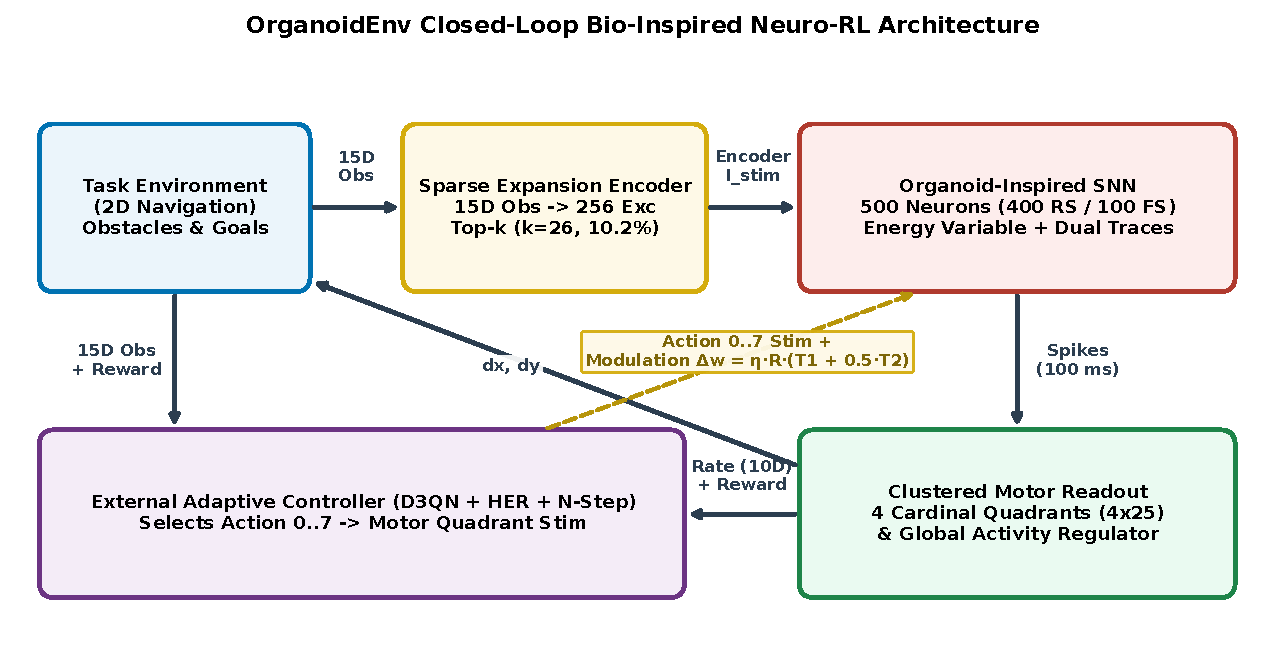
\includegraphics[width=0.92\textwidth]{fig01_architecture_loop.pdf}
\caption{OrganoidEnv closed-loop architecture. The 15-dimensional environment observation is routed simultaneously to the external D3QN agent and the top-$k$ sparse expansion encoder ($256$ RS units). The controller selects a directional action, stimulating one of four $25$-neuron motor quadrants with $+20.0$ current for $100\text{ ms}$. Differential motor quadrant spiking drives continuous coordinate displacement in the Gymnasium arena. The Global Activity Regulator (GAR) and metabolic governor constrain dynamical stability, while a presynaptic dual-trace three-factor rule updates recurrent synaptic weights based on scalar reward $R_t$.}
\label{fig:arch}
\end{figure*}

\subsection{Controller-SNN Interface and Action Conversion}
The control interface operates in discrete $100\text{ ms}$ steps. At each step, the environment provides a $15$-dimensional continuous state vector $\mathbf{s}_t \in \mathbb{R}^{15}$ (agent coordinates, target coordinates, context bit, four-way proximity sensors, velocities, and normalized offsets). The external D3QN agent processes $\mathbf{s}_t$ and outputs a discrete action $a_t \in \{0, 1, 2, 3\}$ corresponding to cardinal directions: $\texttt{Up}$ ($400..424$), $\texttt{Down}$ ($425..449$), $\texttt{Left}$ ($450..474$), and $\texttt{Right}$ ($475..499$).

The SNN converts this discrete action into physical arena movement via population decoding. Over the $100\text{ ms}$ interval ($1000$ integration ticks at $dt = 0.1\text{ ms}$), the chosen motor quadrant receives direct external stimulation ($I_i \mathrel{+}= 20.0$), driving recurrent and lateral firing. Cursor displacement is decoded from the spike count difference between opponent quadrants:
\begin{equation}
\Delta x = 0.05 \left(N_{\mathrm{right}} - N_{\mathrm{left}}\right), \quad \Delta y = 0.05 \left(N_{\mathrm{up}} - N_{\mathrm{down}}\right).
\label{eq:motor_displacement}
\end{equation}
Crucially, learning occurs simultaneously across two levels:
\begin{enumerate}
    \item \textbf{External Controller:} The D3QN neural network updates its parameters via gradient descent on the temporal-difference (TD) Bellman error, learning which quadrant to stimulate based on the global state.
    \item \textbf{Recurrent SNN Plant:} Synaptic weights $w_{ij}$ within the SNN update locally via reward-modulated three-factor plasticity based on task reward $R_t$.
\end{enumerate}

\subsection{Metabolic-Izhikevich Neuron Dynamics}
Neuron dynamics follow Euler integration ($dt = 0.1\text{ ms}$) of the two-dimensional Izhikevich system~\cite{Izhikevich2003simple}, augmented with a normalized intracellular energy variable $E_i \in [-0.10, 1.0]$, an absolute refractory period $t_{\mathrm{ref}} = 2.0\text{ ms}$, and numerical voltage clipping $v_i^c = \mathrm{clip}(v_i, -100.0, +60.0)$:
\begin{align}
\frac{dv_i}{dt} &= \mathbb{I}[E_i > 0]\left(0.04 (v_i^c)^2 + 5.0 v_i^c + 140.0 - u_i + I_i\right) \nonumber \\
                &\quad + \mathbb{I}[E_i \le 0]\left(\frac{-80.0 - v_i^c}{0.5\text{ ms}}\right), \label{eq:dv} \\
\frac{du_i}{dt} &= a_i\left(b_i v_i^c - u_i\right), \label{eq:du} \\
\frac{dE_i}{dt} &= \frac{1.0 - E_i}{\tau_{\mathrm{rec}, i}}. \label{eq:dE}
\end{align}
Here, $v_i, u_i, I_i$, and $w_{ij}$ are expressed in standard dimensionless Izhikevich units. Synaptic transmission is modeled as instantaneous delta-jump current transients ($I_i \mathrel{+}= w_{ij}$ on presynaptic spike arrival). Excitatory Regular Spiking (RS) neurons use parameters $(a, b, c, d) = (0.02, 0.2, -65.0, 8.0)$ and recovery constant $\tau_{\mathrm{rec,exc}} = 1000\text{ ms}$; Fast Spiking (FS) inhibitory interneurons use $(0.1, 0.2, -65.0, 2.0)$ and $\tau_{\mathrm{rec,inh}} = 500\text{ ms}$.

A spike is emitted when $v_i \ge 30.0$ and $E_i > 0$. Upon spiking, state variables reset: $v_i \leftarrow c_i$, $u_i \leftarrow u_i + d_i$, and energy decreases by a fixed metabolic increment:
\begin{equation}
E_i \leftarrow E_i - \Delta_E, \quad \Delta_E = 0.10.
\label{eq:E_deplete}
\end{equation}
Because emission strictly requires $E_i > 0$, the post-spike energy is lower-bounded by $\approx -0.10$. When $E_i \le 0$, the active depolarization term in Eq.~\eqref{eq:dv} is extinguished, and an energetic clamp pulls the membrane toward $-80.0$ with a fast time constant of $0.5\text{ ms}$, modeling the hyperpolarizing action of ATP-sensitive potassium ($\mathrm{K}_{\mathrm{ATP}}$) channels~\cite{Tanner2011}.

\textbf{Proposition 1 (Asymptotic Steady-State Firing Rate Ceiling):}
Consider a neuron firing at a sustained mean rate $f$ (in Hz). In each second, metabolic depletion is $\Delta_E \cdot f$. At steady state ($dE/dt = 0$), equating average depletion to continuous linear recovery $(1 - \bar{E}) / \tau_{\mathrm{rec}}$ yields:
\begin{equation}
\bar{E} = 1.0 - \Delta_E \cdot f \cdot \tau_{\mathrm{rec}}.
\label{eq:E_ss}
\end{equation}
Because sustained firing requires $\bar{E} > 0$, the maximum sustained firing rate cannot exceed:
\begin{equation}
f_{\max} = \frac{1.0}{\Delta_E \cdot \tau_{\mathrm{rec}}}.
\label{eq:f_max}
\end{equation}
For excitatory units ($\Delta_E = 0.10, \tau_{\mathrm{rec}} = 1.0\text{ s}$), $f_{\max,\mathrm{exc}} = 10.0\text{ Hz}$; for inhibitory units ($\Delta_E = 0.10, \tau_{\mathrm{rec}} = 0.5\text{ s}$), $f_{\max,\mathrm{inh}} = 20.0\text{ Hz}$. In an $80/20$ recurrent network, the population-weighted theoretical ceiling is $0.8(10.0) + 0.2(20.0) = 12.0\text{ Hz}$.

\emph{Transient Qualification:} $f_{\max}$ is strictly an asymptotic bound ($t \to \infty$, $dE/dt = 0$). In finite-horizon runs, the initial energy reserve ($E_0 = 1.0$ permits roughly $1/\Delta_E = 10$ spikes per neuron before depletion) and GAR coma kicks allow transient rates above $f_{\max}$. In our parameter sweep (Fig.~\ref{fig:sensitivity_sweep}A) the excess reached about $25\%$ (e.g., $\approx 3.1\text{ Hz}$ at $\Delta_E = 0.20$, $\tau_{\mathrm{rec}} = 2000\text{ ms}$, where $f_{\max} = 2.5\text{ Hz}$). Convergence of long-horizon rates to Eq.~\eqref{eq:f_max} is expected but was not measured here (Section~\ref{sec:discussion}).

\subsection{Anatomical Compartments and Dale's Principle}
Network connectivity strictly enforces Dale's principle with non-negative synaptic weights $w_{ij} \ge 0$. Excitatory units deliver depolarizing post-synaptic current jumps ($+w_{ij}$); inhibitory units deliver hyperpolarizing jumps ($-w_{ij}$). The $500$ neurons are organized into five structured compartments:
\begin{enumerate}
    \item \textbf{Sparse Sensory Encoder ($0..255$):} $256$ RS excitatory neurons.
    \item \textbf{Hidden Excitatory Reservoir ($256..299$):} $44$ RS excitatory neurons.
    \item \textbf{Global Inhibitory Population ($300..399$):} $100$ FS inhibitory interneurons.
    \item \textbf{Motor Readout Population ($400..499$):} $100$ RS excitatory neurons divided into four $25$-neuron cardinal directional clusters.
\end{enumerate}
Connection densities and baseline weights ($w_0$) are configured as follows:
\begin{itemize}
    \item $\mathrm{Encoder} \to \mathrm{Hidden}$: $p = 0.15, w_0 = 20.0$ (excitatory).
    \item $\mathrm{Hidden} \to \mathrm{Motor}$: $p = 0.15, w_0 = 20.0$ (excitatory).
    \item $\mathrm{Hidden} \to \mathrm{Hidden}$: $p = 0.05, w_0 = 10.0$ (excitatory recurrent).
    \item $\mathrm{Motor} \to \mathrm{Motor}$: $p = 0.10, w_0 = 10.0$ (lateral excitatory).
    \item $\mathrm{Inhibitory} \to \mathrm{All}$: $p = 0.10, w_0 = 25.0$ (global feedback inhibition).
\end{itemize}
All neurons receive independent Poisson background excitation at $10\text{ Hz}$ with amplitude $w_{\mathrm{bg}} = 4.0$. Note that the $256$ sensory input channels project onto only $44$ hidden excitatory units, forming a severe anatomical bottleneck that constrains internal recurrent representations.

\subsection{Global Activity Regulator (GAR) and Inhibitory Scaling}
At the conclusion of each $100\text{ ms}$ step, the Global Activity Regulator (GAR) tallies $N_{\mathrm{recent}}$, defined as the total population spike count across all $500$ neurons during the preceding $100\text{ ms}$ window ($\Delta t = 0.1\text{ s}$). GAR executes tri-state supervisory control:
\begin{enumerate}
    \item \textbf{Safety Reset:} If numerical corruption occurs ($v_i$ is NaN or infinite), potentials are reset ($v_i \leftarrow -65.0\text{ mV}, E_i \leftarrow 1.0$).
    \item \textbf{Coma Kick ($N_{\mathrm{recent}} < 50$):} If mean population firing drops below $1.0\text{ Hz}$ ($<50$ spikes across $500$ neurons over $100\text{ ms}$), stochastic depolarizing current $I_i \leftarrow 5.0 \cdot \mathcal{U}(0, 1)$ is injected across all neurons to prevent quiescent arrest.
    \item \textbf{Seizure Clamp ($N_{\mathrm{recent}} > 5000$):} If mean population firing exceeds $100.0\text{ Hz}$ ($>5000$ spikes), excitatory input is silenced ($I_i \leftarrow 0$), membranes are hyperpolarized ($v_i \leftarrow \min(v_i, -70.0\text{ mV})$), and inhibitory feedback weights are potentiated by $+2.0$.
\end{enumerate}
Across all $55{,}000$ spiking-network training episodes ($11$ unique spiking conditions $\times 10$ seeds $\times 500$ episodes), $0$ seizure clamps and $0$ safety resets were triggered, while $44{,}933$ coma kicks occurred across the $45{,}000$ GAR-enabled episodes ($\approx 0.999$/episode, exclusively at step $0$ because the reset integrates for only $10\text{ ms}$ and produces $<50$ initial spikes; $0$ in C4 and B3). Thus, in nominal closed-loop operation GAR acts as a dormant guardrail rather than an active dynamical driver; its effect under extreme drive is examined in the stability sweep (Fig.~\ref{fig:phase}).

Between episodes, homeostatic synaptic scaling adjusts the global feedback inhibitory weight $w_{\mathrm{inh}}$ toward a target E/I ratio of $1.5$:
\begin{equation}
\Delta w_{\mathrm{inh}} = 0.10 \left(1.5 \bar{w}_{\mathrm{exc}} - w_{\mathrm{inh}}\right),
\label{eq:ei_scaling}
\end{equation}
stabilizing long-term network excitability.

\subsection{Presynaptic Dual-Trace Three-Factor Plasticity and Pruning}
To achieve credit assignment without non-causal backpropagation, synapses maintain two presynaptic eligibility traces: a fast behavioral trace ($\tau_1 = 100\text{ ms}$) and a slow multi-second consolidation trace ($\tau_2 = 2500\text{ ms}$). When a presynaptic spike arrives, both traces increment: $\text{Trace1}_{ij} \leftarrow \text{Trace1}_{ij} + 1.0$, $\text{Trace2}_{ij} \leftarrow \text{Trace2}_{ij} + 1.0$. In the absence of spikes, traces decay exponentially:
\begin{equation}
\frac{d\,\text{Trace1}_{ij}}{dt} = -\frac{\text{Trace1}_{ij}}{\tau_1}, \quad \frac{d\,\text{Trace2}_{ij}}{dt} = -\frac{\text{Trace2}_{ij}}{\tau_2}.
\label{eq:traces}
\end{equation}
Synaptic weights relax weakly toward baseline $w_0$ with time constant $\tau_{\mathrm{decay}} = 10\text{ s}$. At the end of each step, task reward $R_t$ modulates synaptic updates via a three-factor rule:
\begin{equation}
\Delta w_{ij} = \eta_{\mathrm{DA}} R_t \left(\text{Trace1}_{ij} + 0.5\,\text{Trace2}_{ij}\right),
\label{eq:three_factor}
\end{equation}
with dopamine learning rate $\eta_{\mathrm{DA}} = 0.01$ and clipping to $[0.0, 100.0]$. This rule is strictly presynaptic (independent of post-synaptic spike timing) and is loosely inspired by synaptic tagging and capture~\cite{Frey1997SynapticTagging}. Every $10$ episodes, activity-dependent structural pruning sets persistently weak weights ($w_{ij} < 0.1$) to zero~\cite{Navlakha2015Pruning}.

\subsection{Sparse Expansion Sensory Encoder}
The continuous $15\text{D}$ observation $\mathbf{s}_t$ is projected into the $256$-channel input layer via a fixed random weight matrix $W_{\mathrm{SDM}} \in \mathbb{R}^{256 \times 15}$ with entries drawn from $\mathcal{N}(0, 1)$. To ensure sparse coding inspired by Sparse Distributed Memory~\cite{Kanerva1988SDM} and expansion theory~\cite{Babadi2014Sparse}, only the top-$k = 26$ units with the largest projections receive $+20.0$ depolarizing stimulation during the step, enforcing an active budget of exactly $26/256 \approx 10.2\%$ by mathematical construction.

\section{Experimental Design and Methodology}
\label{sec:experimental_design}

\subsection{Curriculum and Multi-Seed Protocol}
We evaluate OrganoidEnv in a continuous 2D arena $[0, 1]^2$ over a four-stage navigation curriculum ($500$ episodes $\times 80$ maximum steps per episode):
\begin{itemize}
    \item \textbf{Stage 1 (Episodes 0--99):} Open arena without obstacles, goal radius $r_{\mathrm{goal}} = 0.15$.
    \item \textbf{Stage 2 (Episodes 100--199):} Static circular and rectangular obstacles, $r_{\mathrm{goal}} = 0.10$.
    \item \textbf{Stage 3 (Episodes 200--349):} Dual-target context switching (target indicator bit toggled), $r_{\mathrm{goal}} = 0.10$.
    \item \textbf{Stage 4 (Episodes 350--499):} Full-precision navigation, $r_{\mathrm{goal}} = 0.05$, step penalty $-0.05$, collision penalty $-15.0$, goal bonus $+50.0$, waypoint bonus $+5.0$, exploration bonus $+0.5$, and near-miss bonus $+1.0$.
\end{itemize}

To guarantee statistical rigor, all experimental conditions are evaluated across $n = 10$ equalized random seeds: \texttt{[42, 123, 456, 789, 1024, 2024, 3033, 4044, 5055, 6066]}. Phase A diagnostic audits confirmed that earlier preliminary $5$-seed runs formed an exact strict proper subset of these $10$ seeds.

\subsection{Experimental Conditions and Baselines}
We investigate the full OrganoidEnv model (\textbf{C0}) against nine mechanistic ablations and eight algorithmic baseline configurations ($18$ conditions in total, $180$ training runs):
\begin{itemize}
    \item \textbf{C1 (Frozen Weights):} Synaptic plasticity disabled ($\Delta w_{ij} = 0$).
    \item \textbf{C2 (Random SNN):} Fixed random weights throughout training.
    \item \textbf{C3 (No Metabolism, GAR on):} Metabolic fatigue disabled ($\Delta_E = 0, E_i = 1.0$) with GAR enabled.
    \item \textbf{C4 (No GAR):} Tri-state regulator and E/I scaling disabled.
    \item \textbf{C5 (No Pruning):} Structural synaptic pruning disabled.
    \item \textbf{C6 (Single Trace, 50 ms):} Single presynaptic eligibility trace with $\tau = 50\text{ ms}$.
    \item \textbf{C6b (Single Trace, 100 ms):} Single eligibility trace with $\tau = 100\text{ ms}$ and full weighting ($1.0$).
    \item \textbf{C6c (Single Trace, 2500 ms):} Single eligibility trace with $\tau = 2500\text{ ms}$ and half weighting ($0.5$).
    \item \textbf{C8 (Unregulated: No GAR, No Metabolism):} Both metabolic fatigue and GAR disabled ($\Delta_E = 0$, $E_i = 1.0$, GAR off).
    \item \textbf{B1 / B1b (Direct D3QN):} D3QN controlling \texttt{SkeletonEnv} at step size $0.25$ (B1) and step size $0.05 \le r_{\mathrm{goal}}$ (B1b).
    \item \textbf{B2 / B2b (Standard MLP-DQN):} Standard MLP-DQN on \texttt{SkeletonEnv} at step size $0.25$ (B2) and step size $0.05$ (B2b).
    \item \textbf{B3 (Canonical LIF):} Leaky Integrate-and-Fire reservoir (\texttt{SimpleSNNEnv}).
    \item \textbf{B4 / B4b (PPO):} Stable-Baselines3 PPO on \texttt{SkeletonEnv} at step size $0.25$ (B4) and step size $0.05$ (B4b).
    \item \textbf{B5 (Random Policy):} Uniform random action selection on OrganoidEnv.
\end{itemize}
A condition with GAR on and metabolism off was originally planned as a separate ``GAR-only'' condition (C7); it is identical to C3 and is therefore reported once, while C8 provides the unregulated (GAR-off, metabolism-off) training control. Comparing step $0.25$ (B1, B2, B4) against step $0.05$ (B1b, B2b, B4b) directly resolves the Stage-4 goal-diameter ($0.10$) step-size confound.

\subsection{Mathematical Formulations of Metrics}
All metrics are computed over late-stage performance (episodes 401--500) with exploration noise disabled:
\begin{enumerate}
    \item \textbf{Episodic Return:} $G = \sum_{t=0}^{T} R_t$.
    \item \textbf{Shifted Return per 1000 Spikes:} To avoid negative ratios, returns are shifted by a constant $+250.0$ (chosen so that all spiking-condition mean returns are positive):
    \begin{equation}
    U = \frac{\bar{G} + 250.0}{\bar{S}_{\mathrm{total}} / 1000.0},
    \label{eq:utility}
    \end{equation}
    where $\bar{S}_{\mathrm{total}}$ is the total spikes emitted by the network during the episode. Because $U$ depends on the arbitrary offset, it is a descriptive indicator only and not an information-theoretic efficiency.
    \item \textbf{Directional Selectivity Index (DSI):} Evaluated by stimulating each motor quadrant independently with $+25.0$ probe current and recording mean firing rates $r_{\mathrm{up}}, r_{\mathrm{down}}, r_{\mathrm{left}}, r_{\mathrm{right}}$:
    \begin{equation}
    \begin{aligned}
    \text{DSI} = \max\Biggl( & \frac{|r_{\mathrm{up}} - r_{\mathrm{down}}|}{r_{\mathrm{up}} + r_{\mathrm{down}} + 10^{-9}}, \\
    & \frac{|r_{\mathrm{left}} - r_{\mathrm{right}}|}{r_{\mathrm{left}} + r_{\mathrm{right}} + 10^{-9}} \Biggr).
    \end{aligned}
    \label{eq:dsi}
    \end{equation}
    Because the probe stimulates a motor quadrant directly, DSI also reflects the stimulation response and recurrent leakage, not only learned tuning (Section~\ref{sec:results}).
    \item \textbf{Lag-1 Branching Ratio ($\sigma$):} Computed over $4\text{ ms}$ population spike-count bins $A_t$:
    \begin{equation}
    \sigma = \max\left(0, \frac{\mathrm{Cov}(A_{t+1}, A_t)}{\mathrm{Var}(A_t)}\right).
    \label{eq:branching}
    \end{equation}
    Lag-1 branching estimators depend on bin width and are biased downward under subsampling relative to multi-step regression~\cite{Wilting2018Criticality}; we use $\sigma$ solely to compare conditions, not as an absolute criticality measure.
    \item \textbf{Avalanche Size Exponent ($\alpha$):} Maximum-likelihood estimate following Clauset et al.~\cite{Clauset2009PowerLaw}, with fixed $S_{\min} = 2$:
    \begin{equation}
    \alpha = 1 + N_{\mathrm{av}} \left[\sum_{i=1}^{N_{\mathrm{av}}} \ln\left(\frac{S_i}{S_{\min} - 0.5}\right)\right]^{-1}.
    \label{eq:alpha}
    \end{equation}
    Discrete Kolmogorov--Smirnov (KS) bootstrap goodness-of-fit tests ($100$ resamples) and log-likelihood ratio (LLR) comparisons against a discrete exponential distribution rejected an unbounded power law ($p_{\mathrm{gof}} = 0.0$, $\mathrm{LLR} < 0$, $p < 10^{-15}$ across all tested conditions), so $\alpha$ is reported purely as a descriptive tail-slope summary.
    \item \textbf{Fano Factor:} $\mathrm{FF} = \mathrm{Var}(C) / \mathrm{Mean}(C)$, computed over $4\text{ ms}$ population spike count bins.
\end{enumerate}

Statistical comparisons report \texttt{rliable} Interquartile Means (IQM) with $95\%$ stratified bootstrap confidence intervals ($5000$ resamples)~\cite{Agarwal2021rliable}, two-sided Mann--Whitney U tests with Benjamini--Hochberg FDR adjustments ($p_{\mathrm{FDR}}$), and rank-biserial effect sizes ($r_{\mathrm{rb}}$).

\section{Empirical Results}
\label{sec:results}

\subsection{Biophysical Dynamics and Neural Avalanche Statistics}
Fig.~\ref{fig:biophys} displays the electrophysiological profile of C0 during Stage-4 navigation. Under continuous closed-loop drive, the population maintains an operational firing rate of $6.51\text{ Hz}$ IQM [$5.53, 7.29$] and a mean cellular energy level of $\bar{E} = 0.586$ [$0.565, 0.612$]. This rate lies within the $2\text{--}20\text{ Hz}$ working target band we adopt for mean population rates; the band is a modeling assumption, not a fit to specific organoid measurements~\cite{Trujillo2019CellStemCell}.

\begin{figure*}[t]
\centering
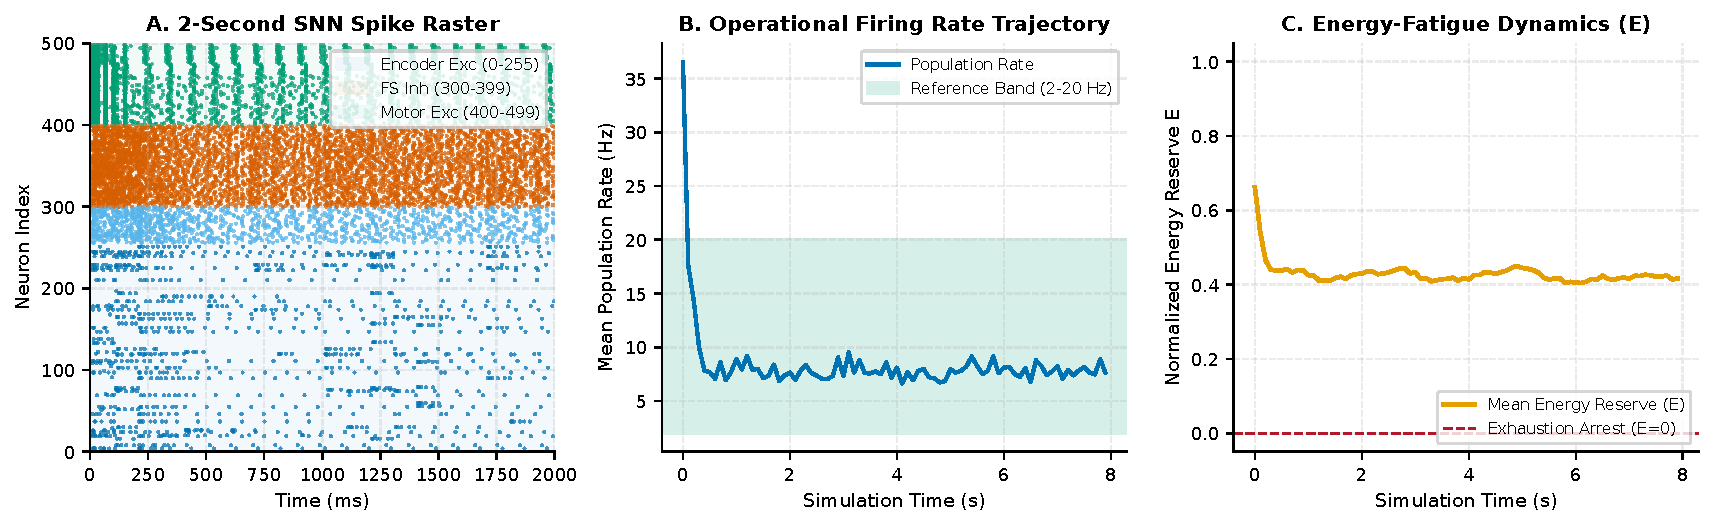
\includegraphics[width=0.95\textwidth]{fig02_biophysical_electrophysiology.pdf}
\caption{Biophysical characterization during Stage-4 evaluation (representative run): (A) $2\text{ s}$ spike raster partitioned into Encoder, Hidden, FS Inhibitory, and Motor compartments; (B) population-rate trajectory, with an initial transient from the full energy reserve; (C) mean energy reserve $E(t)$ of the same run. The cross-seed IQM values are $6.51\text{ Hz}$ and $\bar{E} = 0.586$ (Table~\ref{tab:results}); the shaded band is the $2\text{--}20\text{ Hz}$ working target band.}
\label{fig:biophys}
\end{figure*}

\begin{figure}[t]
\centering
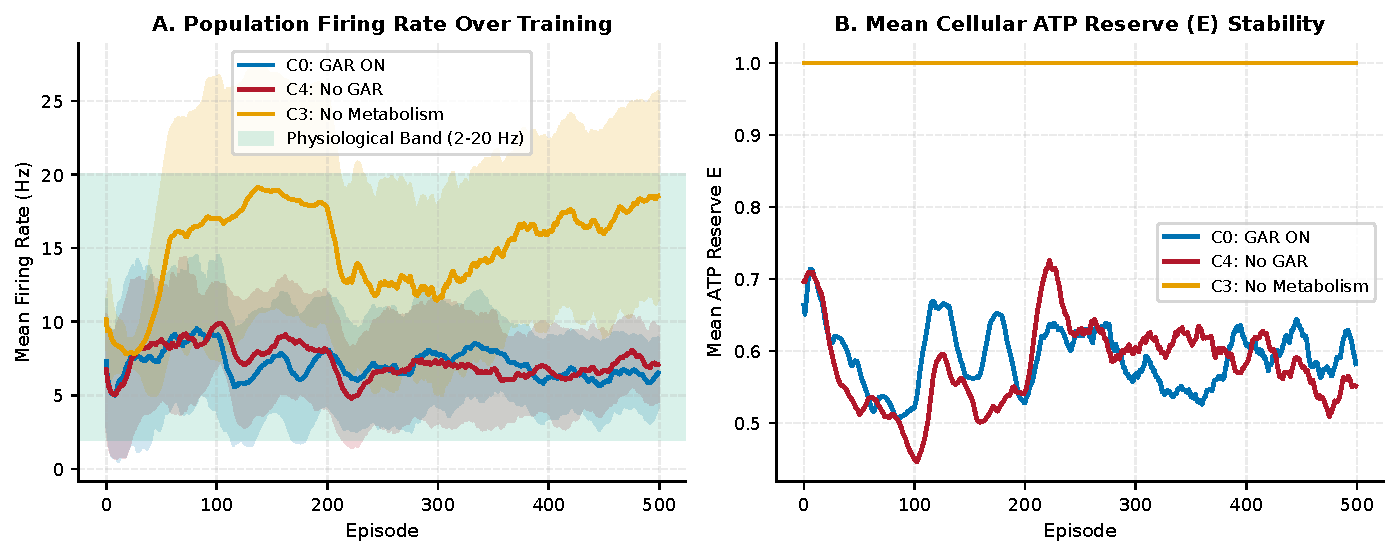
\includegraphics[width=\columnwidth]{fig04_gar_homeostasis.pdf}
\caption{Closed-loop activity across training episodes comparing C0 (Full Model), C4 (No GAR), and C3 (No Metabolism). C0 and C4 are indistinguishable. Disabling metabolism (C3) raises rates ($\sim 17.4\text{ Hz}$, largely inside the $2\text{--}20\text{ Hz}$ band) and keeps energy reserves saturated ($E = 1.0$).}
\label{fig:gar}
\end{figure}

\begin{figure}[t]
\centering
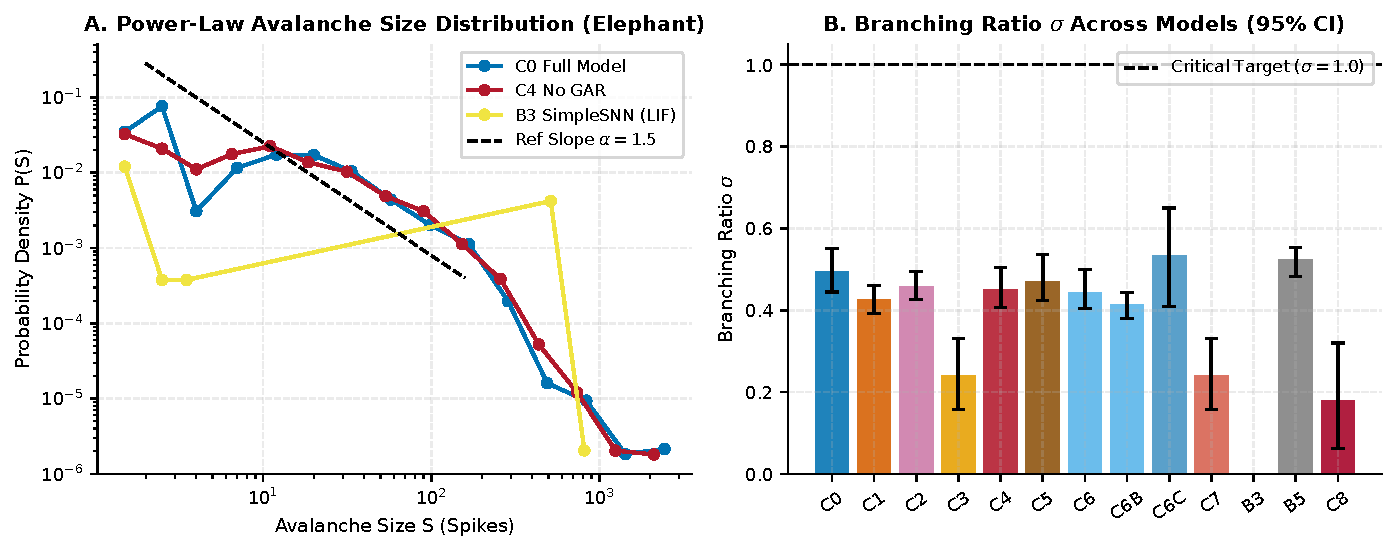
\includegraphics[width=\columnwidth]{fig05_criticality_avalanches.pdf}
\caption{Neural avalanche statistics ($4\text{ ms}$ binning): (A) avalanche-size distribution $P(S)$ with a reference slope of $1.5$; the curves bend and cut off at large $S$ rather than following a clean power law; (B) multistep branching ratio $\sigma_{\mathrm{MR}}$ showing subcritical dynamics ($\sigma_{\mathrm{MR}} \approx 0.49$) across conditions.}
\label{fig:avalanches}
\end{figure}

To describe network dynamics, Fig.~\ref{fig:avalanches} presents avalanche-size distributions~\cite{Beggs2003Avalanches} ($4\text{ ms}$ binning), with condition-wise metrics in Table~\ref{tab:criticality} (Appendix~\ref{app:criticality}). In C0, the multistep branching ratio is $\sigma_{\mathrm{MR}} = 0.494$ [$0.444, 0.551$], the avalanche size exponent is $\alpha = 1.30$ [$1.29, 1.35$], and the Fano factor is $18.92$. We report these statistics descriptively:
\begin{enumerate}
    \item \textbf{Subcritical Dynamics:} The branching ratio $\sigma_{\mathrm{MR}} \approx 0.494$ is well below the critical value ($\sigma = 1.0$), indicating a stable, strongly subcritical regime.
    \item \textbf{Non-Discriminating Avalanche Exponents:} The exponent $\alpha$ remains approximately $1.30$ across conditions (C0: $1.30$, C1: $1.30$, C2: $1.30$, C4: $1.30$, C6: $1.31$, C8: $1.26$, and the untrained random policy B5: $1.39$). Because $\alpha \approx 1.3$ appears regardless of learning or homeostasis, it reflects fixed network structure and thresholding. Moreover, Clauset et al.\ KS goodness-of-fit tests reject a true power law across all tested conditions ($KS \in [0.317, 0.629]$, $p_{\mathrm{gof}} = 0.0$, $\mathrm{LLR} \le -1396.5$ vs.\ exponential, $p < 10^{-15}$), matching the visible cutoff in Fig.~\ref{fig:avalanches}A.
    \item \textbf{Metabolic Fano Dispersion:} Removing metabolism (C3) raises the Fano factor $6.4\times$ ($121.49$ vs $18.92$ in C0, Table~\ref{tab:criticality}; C8 reaches $107.42$). Its closed-loop rate ($17.41\text{ Hz}$) remains largely inside the $2\text{--}20\text{ Hz}$ band (Fig.~\ref{fig:gar}), so in training the no-metabolism condition is hyperactive and bursty rather than epileptiform; the $>100\text{ Hz}$ regime appears only in the extreme-drive sweep below.
\end{enumerate}

\subsection{2D Stability Phase Space: Isolating Metabolic and Homeostatic Roles}
Fig.~\ref{fig:phase} maps network stability across an external stimulation grid ($I_{\mathrm{stim}} \in [5, 10, 20, 30, 50]$, $w_{\mathrm{inh}} \in [5, 10, 20, 30]$; dimensionless units). Evaluating $80$ configurations ($5\text{ s}$ each) across four control regimes, supplemented by $60\text{ s}$ ($600$-step) long-horizon runs with GAR intervention logging at $(I_{\mathrm{stim}}, w_{\mathrm{inh}}) = (50, 5)$ and $(5, 30)$, isolates the biophysical governor:
\begin{enumerate}
    \item \textbf{Unregulated Regime (GAR OFF, Metabolism OFF):} The $5\text{ s}$ grid-mean rate is $57.38\text{ Hz}$, and the strongest-drive corner ($I_{\mathrm{stim}} = 50$, $w_{\mathrm{inh}} = 5$) reaches $138.64\text{ Hz}$ ($139.06\text{ Hz}$ over $30\text{--}60\text{ s}$), i.e., sustained epileptiform runaway ($>100\text{ Hz}$).
    \item \textbf{GAR-Only Regime (GAR ON, Metabolism OFF):} The $5\text{ s}$ grid-mean rate falls to $47.1\text{ Hz}$ (Fig.~\ref{fig:phase}C) and the maximum to $82.0\text{ Hz}$. In the $60\text{ s}$ run at $(50, 5)$, the mean rate settles at $67.06\text{ Hz}$ ($30\text{--}60\text{ s}$) with $200$ seizure clamps and $200$ coma kicks over $600$ steps, showing that GAR oscillates between clamping runaway excitation and re-igniting quiescent periods without depleting cellular energy.
    \item \textbf{Metabolism-Only Regime (GAR OFF, Metabolism ON):} The $5\text{ s}$ grid-mean rate is $13.85\text{ Hz}$ (range $[12.33, 14.42]\text{ Hz}$), exceeding the asymptotic $12.0\text{ Hz}$ ceiling of Eq.~\eqref{eq:f_max} by $15\text{--}20\%$ due to the initial energy reserve ($E_0 = 1.0$). Over $30\text{--}60\text{ s}$ at $(50, 5)$, the mean rate relaxes from $14.42\text{ Hz}$ ($0\text{--}5\text{ s}$) to $12.46\text{ Hz}$, confirming convergence toward the $12.0\text{ Hz}$ analytic bound.
    \item \textbf{Full Governor (GAR ON, Metabolism ON):} The $5\text{ s}$ grid-mean rate is $13.91\text{ Hz}$ (range $[12.50, 14.45]\text{ Hz}$); over $30\text{--}60\text{ s}$, rates settle to $12.57\text{ Hz}$ at $(50, 5)$ and $12.22\text{ Hz}$ at $(5, 30)$ with $0$ seizure clamps and $1$ step-0 coma kick.
\end{enumerate}
These results indicate that metabolic fatigue is the primary mechanism bounding rates in this sweep, whereas GAR has a measurable effect only when metabolism is disabled and drive is extreme.

\begin{figure*}[t]
\centering
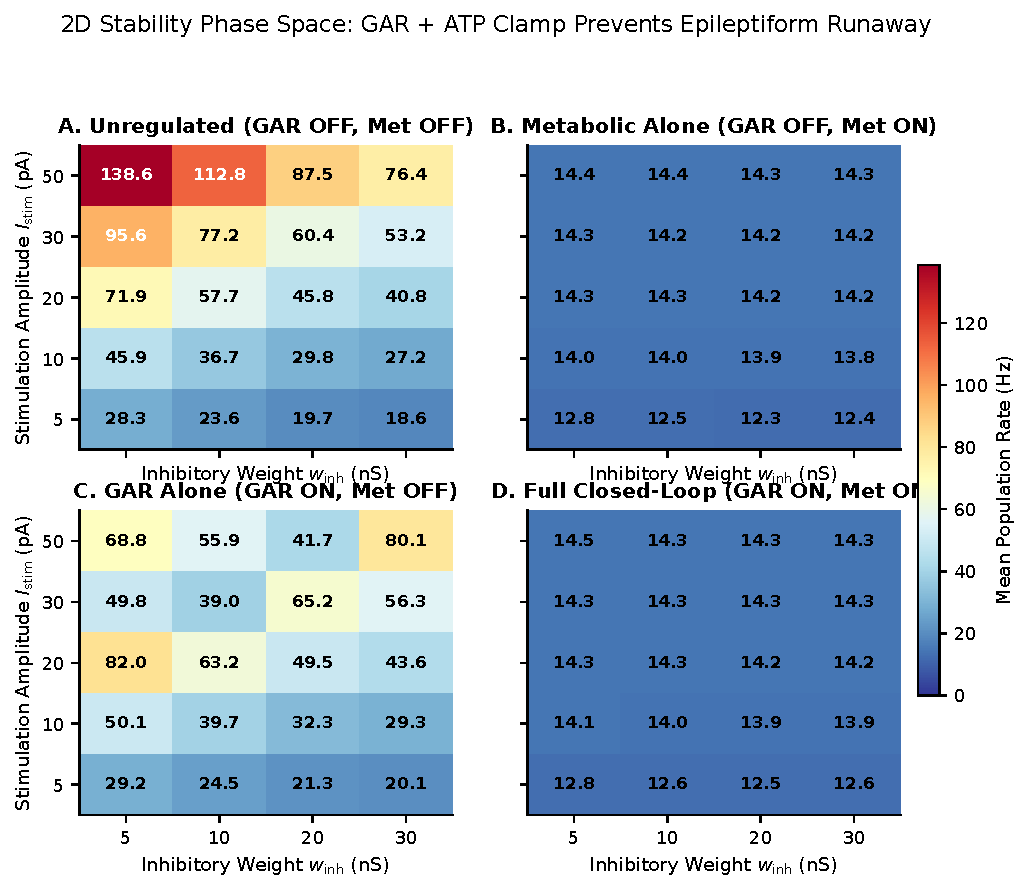
\includegraphics[width=0.95\textwidth]{fig06_stability_phase_space.pdf}
\caption{Empirical 2D stability phase space across $I_{\mathrm{stim}} \times w_{\mathrm{inh}}$ (dimensionless units; $20$ grid points $\times 5\text{ s}$ per regime). Unregulated networks exceed $100\text{ Hz}$ under strong drive. Metabolic fatigue holds $5\text{ s}$ mean rates to $12.3\text{--}14.4\text{ Hz}$ (asymptotic ceiling $12.0\text{ Hz}$); GAR alone reduces but does not bound extreme-drive rates.}
\label{fig:phase}
\end{figure*}

\subsection{Directional Tuning and Plasticity Attribution}
Fig.~\ref{fig:dsi} and Fig.~\ref{fig:plasticity} show motor-cluster selectivity and synaptic weights.

\begin{figure}[t]
\centering
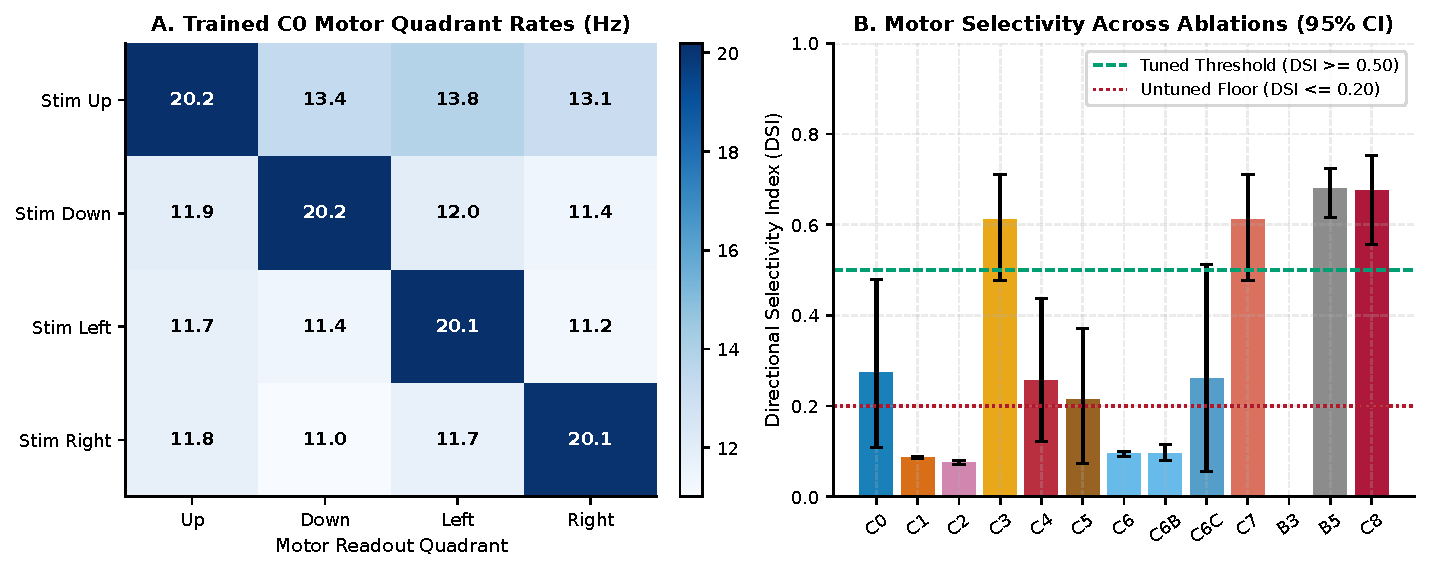
\includegraphics[width=\columnwidth]{fig07_directional_selectivity.pdf}
\caption{(A) C0 $4 \times 4$ motor-quadrant rate matrix under single-quadrant probe stimulation; (B) Directional Selectivity Index (DSI) IQM across conditions with $95\%$ bootstrap CIs. Dashed lines are illustrative reference levels ($0.20$, $0.50$), not statistical thresholds. DSI is highest for the random policy (B5) and the no-metabolism condition (C3) and does not track task performance.}
\label{fig:dsi}
\end{figure}

\begin{figure}[t]
\centering
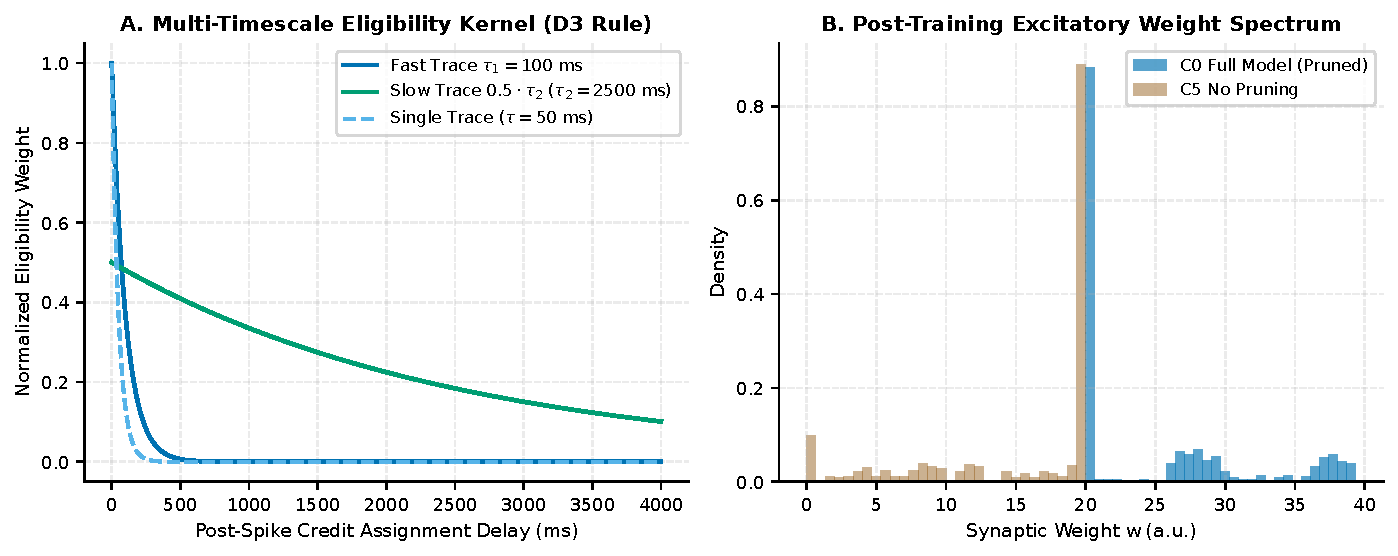
\includegraphics[width=\columnwidth]{fig08_dual_trace_plasticity.pdf}
\caption{(A) Dual-trace eligibility kernel ($\tau_1 = 100\text{ ms}$, $\tau_2 = 2500\text{ ms}$, slow-trace weight $0.5$) versus the $50\text{ ms}$ single-trace kernel of C6; (B) post-training excitatory weight spectrum in C0 (pruned) versus C5 (no pruning); most C0 weights remain near the initial value $w_0 = 20$ (dimensionless units).}
\label{fig:plasticity}
\end{figure}

\emph{DSI does not measure learned tuning.} The uniform random policy (B5) exhibits the highest nominal DSI ($\mathrm{DSI}_{\mathrm{IQM}} = 0.680$ [$0.574, 0.758$]), and the no-metabolism condition C3 reaches $0.611$, both above C0 ($0.275$ [$0.109, 0.480$]). In Fig.~\ref{fig:dsi}A the stimulated quadrant fires at about $20\text{ Hz}$ and the others at $11\text{--}14\text{ Hz}$, so the matrix largely reflects the probe itself. Across plasticity conditions, DSI is highest where the slow trace is active (C0, C4, C5, C6c: $0.22\text{--}0.28$) and lowest in fast-trace-only and static conditions (C1, C2, C6, C6b: $0.08\text{--}0.10$), yet the high-DSI conditions also have the lowest goal rates ($24.7\text{--}41.8\%$ versus $53.7\text{--}63.0\%$). We therefore report DSI descriptively and make no claim that plasticity learns directional tuning.

\emph{Single-Trace Ablations (C6b vs C6c):}
\begin{itemize}
    \item \textbf{C6b ($\tau = 100\text{ ms}$, weight $1.0$):} return IQM $-0.18$ [$-18.48, 15.75$] and goal rate $55.33\%$, with significantly higher return than C0 ($p_{\mathrm{FDR}} = 0.008$, $r_{\mathrm{rb}} = +0.80$).
    \item \textbf{C6c ($\tau = 2500\text{ ms}$, weight $0.5$):} return IQM $-76.46$ [$-122.76, -30.65$] and goal rate $24.67\%$, not significantly different from C0 ($p_{\mathrm{FDR}} = 0.615$, $r_{\mathrm{rb}} = -0.16$).
\end{itemize}
Because C6c changes both the time constant and the weighting relative to C6b, these data suggest, but do not isolate, an effect of the slow trace on performance.

\emph{Plasticity Attribution:}
Static networks (C1 frozen: $-6.04$; C2 random: $+14.68$) and the fast single trace (C6b: $-0.18$) achieve higher in-distribution return than C0 ($-49.50$; Table~\ref{tab:results}; $p_{\mathrm{FDR}} = 0.025$, $0.003$, $0.007$). In this setup the dual-trace rule therefore does not improve control and appears to degrade it. Diagnostic logging over $10$ Stage-4 episodes confirms large episodic weight drift in plastic networks ($\lVert \Delta w \rVert_2 = 486.0$ per episode in C0 vs $0.0$ in C1) alongside large step displacements (mean $0.692$, max $1.414$). This supports two non-exclusive mechanisms: first, plasticity continuously shifts the plant transfer function while the D3QN learns; second, at presynaptic rate $f$, mean traces scale as $f\tau$, making the slow term $0.5\,\mathrm{Trace}_2$ roughly $12\times$ larger than $\mathrm{Trace}_1$ ($0.5 \cdot 2500/100$) when multiplying unnormalized rewards ($+50$ goal, $-15$ collision). Reward-normalized plasticity remains untested.

\begin{figure*}[t]
\centering
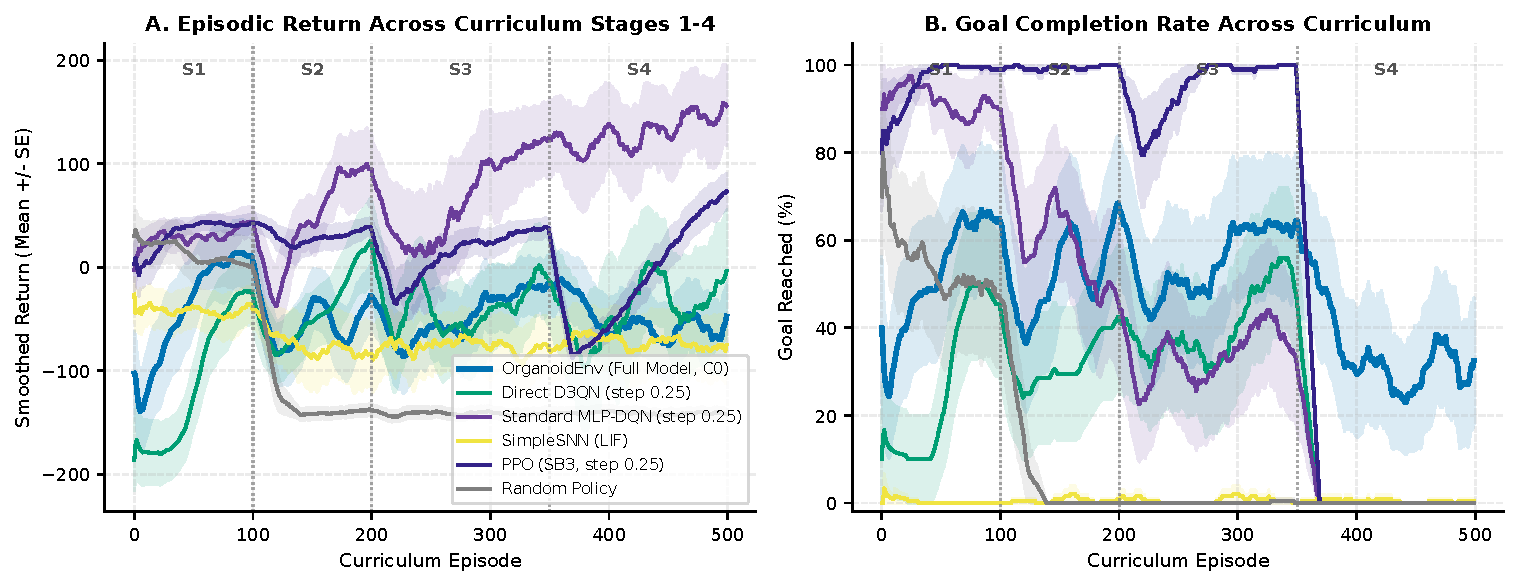
\includegraphics[width=0.92\textwidth]{fig09_learning_curves.pdf}
\caption{Curriculum learning trajectories ($500$ episodes across Stages 1--4; shaded bands show the standard error across $10$ seeds) comparing C0 against direct D3QN, MLP-DQN, SimpleSNN (LIF), PPO, and random baselines. All baselines drop to $0\%$ goal completion shortly after the Stage-4 goal radius shrinks to $0.05$ (episode $350$).}
\label{fig:learning}
\end{figure*}

\begin{figure*}[t]
\centering
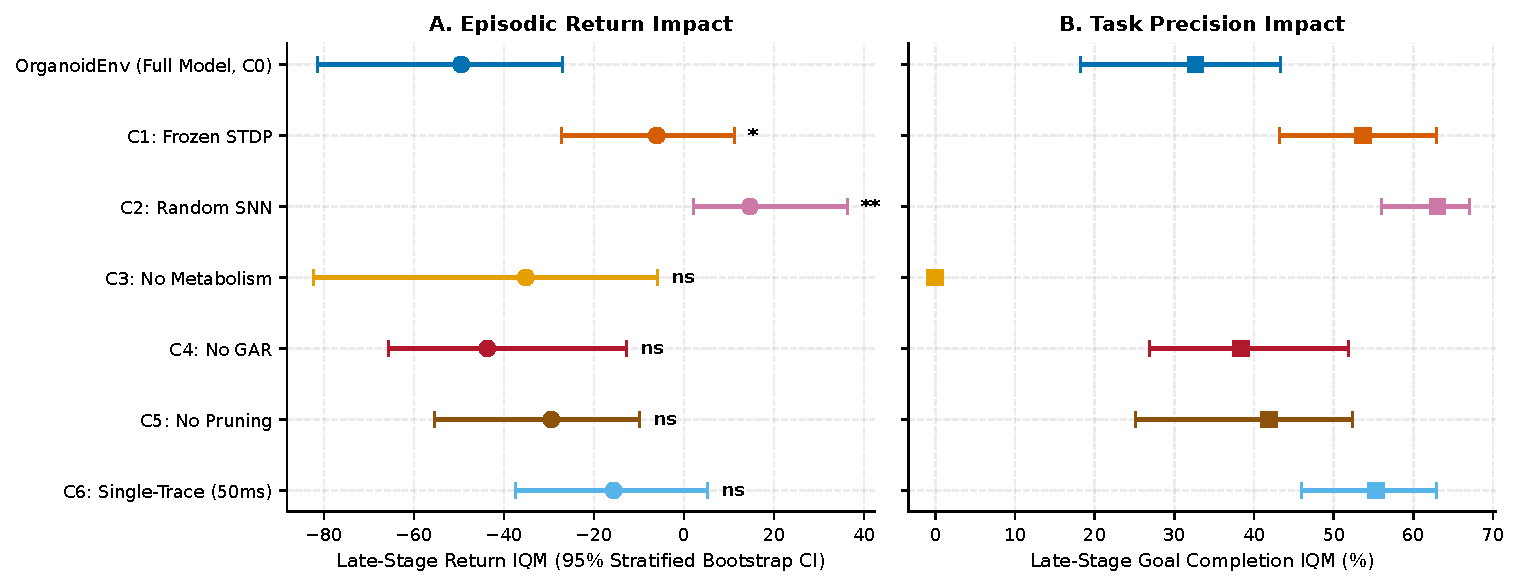
\includegraphics[width=0.92\textwidth]{fig10_ablation_matrix.pdf}
\caption{Ablation forest plot of \texttt{rliable} IQM return (A) and goal-completion IQM (B) with $95\%$ bootstrap CIs; stars mark Benjamini--Hochberg FDR-adjusted Mann--Whitney U significance versus C0 ($*$: $p_{\mathrm{FDR}} < 0.05$, $**$: $p_{\mathrm{FDR}} < 0.01$). C6b, C6c, and the baselines are reported in Table~\ref{tab:results}.}
\label{fig:ablation}
\end{figure*}

\begin{figure}[t]
\centering
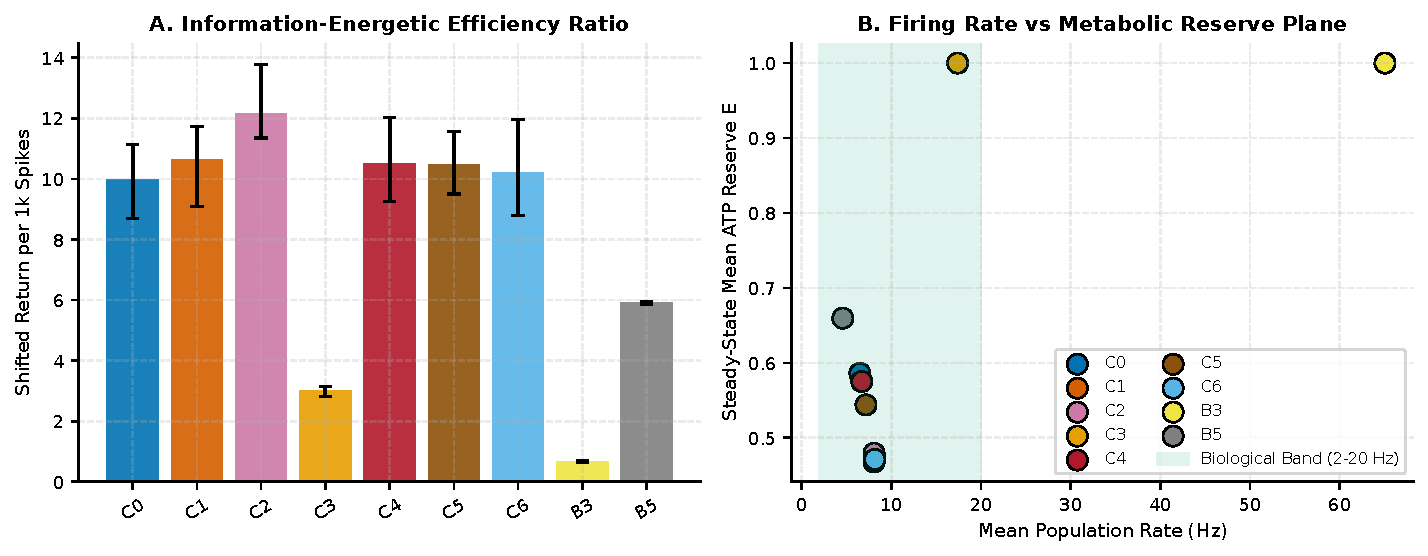
\includegraphics[width=\columnwidth]{fig11_metabolic_efficiency.pdf}
\caption{(A) Shifted return per $1000$ spikes ($+250$ offset; descriptive only, see Section~\ref{sec:experimental_design}) across spiking conditions; (B) mean energy reserve $E$ versus mean population rate.}
\label{fig:efficiency}
\end{figure}

\begin{figure}[t]
\centering
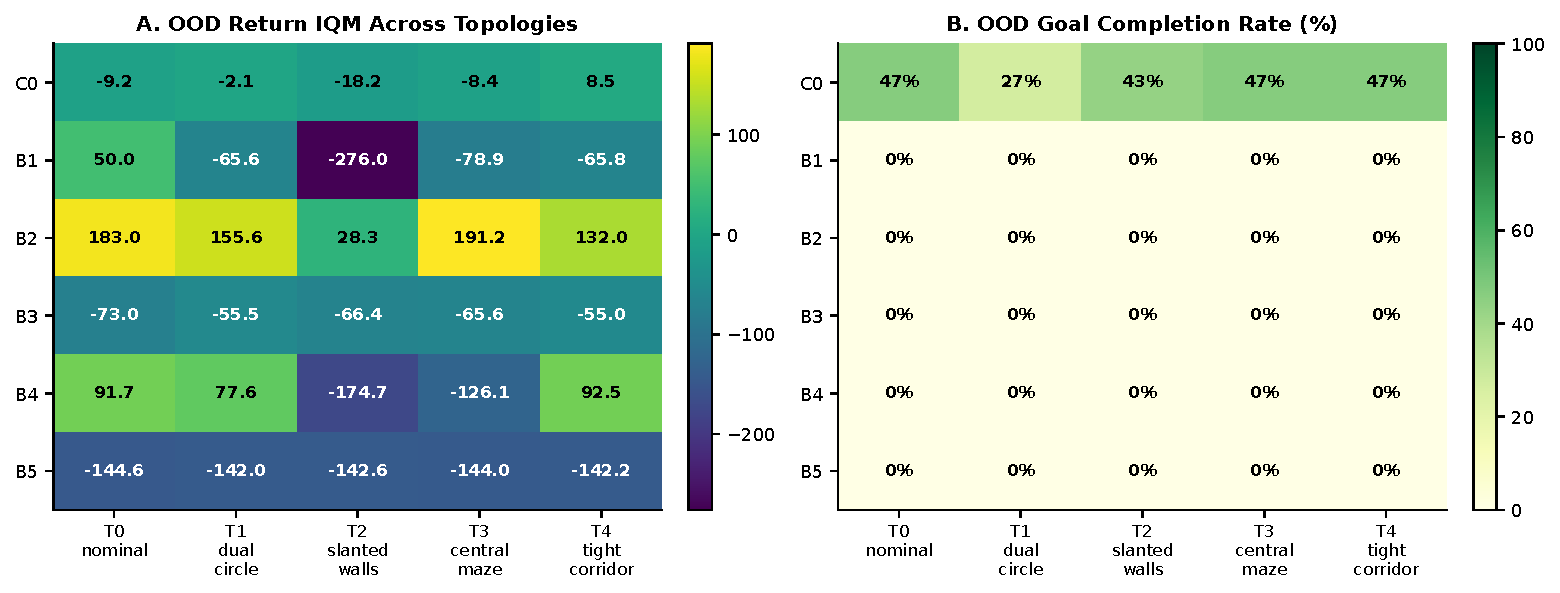
\includegraphics[width=\columnwidth]{fig12_ood_generalization.pdf}
\caption{Zero-shot evaluation across five spatial obstacle topologies (\texttt{T0\_nominal} to \texttt{T4\_tight\_corridor}): return IQM (A) and goal-completion rate (B). Baselines score $0\%$ goal completion in every topology, including the nominal T0, so the comparison does not isolate generalization; B2's positive returns with zero goals reflect shaping bonuses.}
\label{fig:ood}
\end{figure}

\subsection{Curriculum Learning, Energetic Efficiency, and OOD Generalization}
Table~\ref{tab:results} summarizes late-stage performance across all $18$ conditions, while curriculum learning trajectories and ablation results are depicted in Fig.~\ref{fig:learning} and Fig.~\ref{fig:ablation}. Shifted return per spike is shown in Fig.~\ref{fig:efficiency}. Three results emerge:
\begin{enumerate}
    \item \textbf{Metabolic Fatigue and Task Success:} Disabling metabolism (C3: $-35.12$, $0.00\%$ goal; C8 unregulated: $-45.17$, $0.00\%$ goal) eliminates goal completion while firing at $17.00\text{--}17.41\text{ Hz}$, yet returns do not differ significantly from C0 ($-49.50$; $p_{\mathrm{FDR}} = 0.567$ and $0.604$). Stage-4 diagnostic episodes show large opposing-quadrant excursions (mean step displacement $0.727$ in C3 vs $0.692$ in C0; $2.8$ vs $3.2$ collisions/episode), confirming that unthrottled bursts overshoot the $0.05$ goal sphere without completing tasks.
    \item \textbf{Resolving the Baseline Step-Size Confound (0.25 vs 0.05):} At `step = 0.25`, B1, B2, and B4 collapse to $0.00\%$ Stage-4 goal completion because the $0.25$ lattice exceeds the Stage-4 goal diameter ($0.10$), while B2 farms shaping bonuses ($+136.40$ return). When rerun at `step = 0.05` ($\le r_{\mathrm{goal}}$; Table~\ref{tab:results}), all three baselines recover Stage-4 goal completion: **B1b (Direct D3QN)** reaches $26.33\%$ (return $-32.12$, $p_{\mathrm{FDR}} = 0.567$ vs C0), **B2b (MLP-DQN)** reaches $41.67\%$ ($+71.51$, $p_{\mathrm{FDR}} = 0.003$), and **B4b (PPO)** reaches $56.17\%$ ($+59.24$, $p_{\mathrm{FDR}} = 0.002$). This confirms that the earlier $0\%$ Stage-4 collapse was an action-granularity artifact, and that silicon RL baselines match or exceed C0 in-distribution when step sizes are properly matched.
    \item \textbf{Out-of-Distribution Evaluation:} Across unseen obstacle topologies (T0--T4; Table~\ref{tab:ood}, Appendix~\ref{app:ood}), the `step = 0.25` baselines score $0.0\%$ everywhere due to the lattice confound. At `step = 0.05`, B1b ($23.3\%\text{--}40.0\%$), B2b ($8.3\%\text{--}30.0\%$), and B4b ($10.0\%\text{--}25.0\%$) generalize well above zero, though C0 maintains comparable or slightly higher IQMs on four of five topologies ($43.3\%\text{--}46.7\%$ on T0, T2, T3, T4) with overlapping $95\%$ bootstrap CIs.
\end{enumerate}

\begin{table*}[t]
\centering
\caption{Empirical Late-Stage Performance (Last 100 Episodes, $n=10$ seeds each): \texttt{rliable} IQM [95\% Bootstrap CI], Physiology, and Statistical Comparisons vs. C0. B1/B2/B4 use step $0.25$ (confounded); B1b/B2b/B4b use step $0.05 \le r_{\mathrm{goal}}$.}
\label{tab:results}
\resizebox{\textwidth}{!}{%
\begin{tabular}{@{}lcccccc@{}}
\toprule
\textbf{Condition} & \textbf{Return IQM [95\% CI]} & \textbf{Goal Rate (\%)} & \textbf{Rate (Hz)} & \textbf{Mean ATP ($E$)} & \textbf{DSI} & \textbf{$p_{\mathrm{FDR}}$ / $r_{\mathrm{rb}}$ (vs C0)} \\
\midrule
OrganoidEnv (Full Model, C0) & $-49.5\,[-81.5, -27.1]$ & $32.7\%$ $[18.2, 43.3]$ & $6.51$ & $0.586$ & $0.275$ & Reference \\
C1: Frozen STDP & $-6.0\,[-27.1, 11.3]$ & $53.7\%$ $[43.2, 62.8]$ & $8.08$ & $0.468$ & $0.087$ & $0.025$ / $+0.68$ \\
C2: Random SNN & $14.7\,[2.2, 36.4]$ & $63.0\%$ $[56.0, 67.0]$ & $8.09$ & $0.479$ & $0.076$ & $0.003$ / $+0.92$ \\
C3: No Metabolism (GAR on) & $-35.1\,[-82.2, -5.9]$ & $0.0\%$ $[0.0, 0.0]$ & $17.41$ & $1.000$ & $0.611$ & $0.567$ / $+0.20$ \\
C4: No GAR & $-43.7\,[-65.7, -12.8]$ & $38.3\%$ $[26.8, 51.8]$ & $6.72$ & $0.575$ & $0.255$ & $0.734$ / $+0.10$ \\
C5: No Pruning & $-29.5\,[-55.4, -9.9]$ & $41.8\%$ $[25.2, 52.3]$ & $7.18$ & $0.544$ & $0.215$ & $0.362$ / $+0.32$ \\
C6: Single-Trace (50ms) & $-15.6\,[-37.3, 5.2]$ & $55.3\%$ $[46.0, 62.8]$ & $8.17$ & $0.471$ & $0.094$ & $0.051$ / $+0.60$ \\
C6b: Single-Trace Fast (100ms) & $-0.2\,[-18.5, 15.8]$ & $55.3\%$ $[46.3, 63.8]$ & $8.32$ & $0.468$ & $0.095$ & $0.007$ / $+0.80$ \\
C6c: Single-Trace Slow (2500ms) & $-76.5\,[-122.8, -30.6]$ & $24.7\%$ $[11.8, 39.5]$ & $5.87$ & $0.633$ & $0.260$ & $0.604$ / $-0.16$ \\
C8: Unregulated (No GAR, No Met) & $-45.2\,[-123.2, -11.8]$ & $0.0\%$ $[0.0, 0.0]$ & $17.00$ & $1.000$ & $0.675$ & $0.604$ / $+0.16$ \\
B1: Direct D3QN (step 0.25) & $-10.8\,[-72.1, 29.2]$ & $0.0\%$ $[0.0, 0.0]$ & -- & -- & -- & $0.170$ / $+0.44$ \\
B2: Standard MLP-DQN (step 0.25) & $136.4\,[103.9, 169.1]$ & $0.0\%$ $[0.0, 0.0]$ & -- & -- & -- & $0.002$ / $+1.00$ \\
B4: PPO (SB3, step 0.25) & $27.6\,[7.8, 44.9]$ & $0.0\%$ $[0.0, 0.0]$ & -- & -- & -- & $0.002$ / $+0.96$ \\
B1b: Direct D3QN (step 0.05) & $-32.1\,[-85.3, 30.3]$ & $26.3\%$ $[12.8, 52.7]$ & -- & -- & -- & $0.567$ / $+0.20$ \\
B2b: Standard MLP-DQN (step 0.05) & $71.5\,[39.5, 87.3]$ & $41.7\%$ $[20.5, 62.8]$ & -- & -- & -- & $0.003$ / $+0.90$ \\
B4b: PPO (SB3, step 0.05) & $59.2\,[52.8, 71.8]$ & $56.2\%$ $[44.5, 67.0]$ & -- & -- & -- & $0.002$ / $+1.00$ \\
B3: SimpleSNN (LIF) & $-75.0\,[-83.5, -66.1]$ & $0.3\%$ $[0.0, 0.8]$ & $65.06$ & $1.000$ & $0.000$ & $0.160$ / $-0.46$ \\
B5: Random Policy & $-141.5\,[-142.8, -140.4]$ & $0.0\%$ $[0.0, 0.0]$ & $4.60$ & $0.660$ & $0.680$ & $0.007$ / $-0.80$ \\
\bottomrule
\end{tabular}%
}
\end{table*}

\section{Discussion and Limitations}
\label{sec:discussion}

\subsection{Summary of Findings}
Our empirical campaign supports four findings, each qualified below:
\begin{enumerate}
    \item \textbf{Metabolic Rate Limitation:} Energy fatigue yields an analytic asymptotic ceiling ($f_{\max} = 1/(\Delta_E \tau_{\mathrm{rec}})$; $12.0\text{ Hz}$ population-weighted), holds $5\text{ s}$ sweep rates to $12.3\text{--}14.4\text{ Hz}$, and converges over $30\text{--}60\text{ s}$ to $12.2\text{--}12.6\text{ Hz}$ where unregulated networks sustain $139.1\text{ Hz}$.
    \item \textbf{GAR Is Dormant in Training:} Across $55{,}000$ spiking episodes, $0$ seizure clamps and $0$ safety resets fired, and coma kicks occurred only at step 0 ($44{,}933$ total). In the sweep, GAR lowers rates only when metabolism is disabled and drive is extreme (grid mean $47.1$ vs $57.4\text{ Hz}$, oscillating at $67.1\text{ Hz}$ over $60\text{ s}$ with $200$ clamps/kicks), adding nothing measurable on top of metabolism ($13.91$ vs $13.85\text{ Hz}$).
    \item \textbf{Dual-Trace Plasticity Does Not Improve Control Here:} Static networks (C1, C2) and the fast single trace (C6b) achieve higher return than C0 ($p_{\mathrm{FDR}} = 0.025$, $0.003$, $0.007$). Diagnostic logging confirms large weight drift ($\lVert \Delta w \rVert_2 = 486.0$/episode) alongside a $12\times$ slow-trace scale imbalance with unnormalized rewards; reward-normalized updates remain untested.
    \item \textbf{Energy Gating and Task Success:} Disabling energy fatigue (C3, C8) eliminates goal completion ($0.0\%$) at $\sim 17\text{ Hz}$, as unthrottled bursts drive large excursions ($0.727$ mean step displacement) that overshoot the $0.05$ goal sphere.
\end{enumerate}

\subsection{Threats to Validity and Null Results}
We explicitly document negative and null results and design limitations:
\begin{itemize}
    \item \textbf{Structural Pruning (C5):} Removing pruning yields no significant difference in late return ($p_{\mathrm{FDR}} = 0.362$, $r_{\mathrm{rb}} = +0.32$); pruning is an implementation detail rather than a demonstrated functional driver.
    \item \textbf{GAR Removal (C4):} Disabling GAR does not significantly alter late return ($p_{\mathrm{FDR}} = 0.734$, $r_{\mathrm{rb}} = +0.10$), consistent with metabolic fatigue alone being sufficient to stabilize the network in the tested regimes.
    \item \textbf{Non-Discriminating Metrics:} DSI is confounded by the probe stimulus and does not track performance; avalanche exponents fail Clauset power-law goodness-of-fit ($p_{\mathrm{gof}} = 0.0$) and are nearly identical across conditions, while lag-1 branching is subcritical everywhere.
    \item \textbf{Baseline Step-Size Sensitivity:} Rerunning B1, B2, and B4 at `step = 0.05` resolves the `step = 0.25` confound and shows that silicon baselines recover Stage-4 ($26.3\%\text{--}56.2\%$) and OOD ($8.3\%\text{--}40.0\%$) goal completion, outperforming C0 in-distribution on return ($p_{\mathrm{FDR}} \le 0.003$ for B2b/B4b).
    \item \textbf{Reward-Normalization Test:} While episodic $\lVert \Delta w \rVert_2$, step displacement, collisions, $60\text{ s}$ sweeps, and C8 (`GAR-off, Met-off`) were logged and tested, reward-normalized plasticity updates were not run and remain future work.
    \item \textbf{Utility Metric:} The shifted return per spike depends on an arbitrary offset and should not be read as efficiency.
    \item \textbf{Anatomical Bottleneck:} Projecting $256$ sensory input channels onto only $44$ hidden excitatory units imposes a severe informational bottleneck.
    \item \textbf{Lack of Direct Wet-Lab Calibration:} OrganoidEnv is an in silico testbed inspired by cortical organoid physiology; the $2\text{--}20\text{ Hz}$ target band is a modeling assumption, not a fit to organoid recordings.
    \item \textbf{Discrete Time Formulation:} The $100\text{ ms}$ control step abstracts away sub-millisecond spike-timing feedback present in biological closed-loop hardware.
\end{itemize}

\section{Conclusion}
\label{sec:conclusion}
We presented OrganoidEnv, an open, ablatable, Gymnasium-compliant spiking reinforcement learning testbed for studying metabolic and homeostatic constraints in organoid-inspired networks, with a C integration kernel numerically cross-checked against Brian2. Across $18$ conditions and $180$ training runs with $10$ seeds each, plus $5\text{ s}$ and $60\text{ s}$ stability sweeps, we showed that energy fatigue sets an analytic rate ceiling ($12.0\text{ Hz}$) and bounds sweep rates to $12.2\text{--}12.6\text{ Hz}$, that GAR is dormant in training ($0$ seizure clamps across $55{,}000$ episodes) and matters only under extreme drive without metabolism, that the dual-trace plasticity rule did not improve control relative to static or fast-trace networks, and that step-size-matched (`step = 0.05`) silicon baselines match or outperform C0 in-distribution while achieving comparable OOD rates. We document non-discriminating metrics (DSI, power-law $\alpha$) and null ablations (GAR, pruning) plainly to support reproducible research on metabolically constrained spiking control.

\section*{Code and Data Availability}
OrganoidEnv source code, configuration files, seeds, and result tables will be archived at \textcolor{red}{[REPOSITORY URL AND ZENODO DOI]} under \textcolor{red}{[OPEN-SOURCE LICENSE]}.

\bibliographystyle{IEEEtran}
\bibliography{references}

\appendices

\section{RL Controller and Simulation Hyperparameters}
\label{app:hyperparams}
All experiments enforce deterministic multi-engine seeding across \texttt{random}, \texttt{numpy}, \texttt{torch}, and Brian2. The native C integration kernel operates at $dt = 0.1\text{ ms}$ ($1000$ integration steps per $100\text{ ms}$ RL decision interval). Training consists of $500$ episodes with up to $80$ steps ($8.0\text{ s}$ simulated biological time per episode). The D3QN architecture consists of a 2-layer MLP ($128$ units per hidden layer) with NoisyNet linear layers ($\sigma_0 = 0.5$). Training parameters include Adam optimizer with learning rate $\alpha = 3 \times 10^{-4}$, discount factor $\gamma = 0.99$, Polyak target smoothing coefficient $\tau = 0.005$, multi-step return $n_{\mathrm{step}} = 3$, batch size $64$, prioritized experience replay buffer capacity $50{,}000$ (priority exponent $\alpha = 0.6$, importance sampling exponent $\beta = 0.4 \to 1.0$), and Hindsight Experience Replay with future strategy ($k = 4$). The PPO baseline uses Stable-Baselines3 defaults with learning rate $3 \times 10^{-4}$, batch size $64$, and rollout horizon $512$.

\section{Neural Criticality and Spike Dispersion Summary}
\label{app:criticality}
\begin{table}[h]
\centering
\caption{Elephant $4\text{ ms}$-Binned Criticality Metrics (IQM [95\% CI]) Across Spiking Conditions (C3: no metabolism, GAR on)}
\label{tab:criticality}
\resizebox{\columnwidth}{!}{%
\begin{tabular}{@{}lccc@{}}
\toprule
\textbf{Condition} & \textbf{Branching $\sigma_{\mathrm{MR}}$} & \textbf{Avalanche $\alpha$} & \textbf{Fano Factor} \\
\midrule
OrganoidEnv (Full Model, C0) & $0.494$ [$ 0.444, 0.551 $] & $1.30$ [$ 1.29, 1.35 $] & $18.92$ \\
C1 & $0.426$ [$ 0.393, 0.459 $] & $1.31$ [$ 1.30, 1.31 $] & $21.11$ \\
C2 & $0.457$ [$ 0.425, 0.494 $] & $1.30$ [$ 1.29, 1.31 $] & $21.51$ \\
C3 & $0.241$ [$ 0.157, 0.331 $] & $1.25$ [$ 1.24, 1.28 $] & $121.49$ \\
C4 & $0.452$ [$ 0.407, 0.505 $] & $1.31$ [$ 1.29, 1.34 $] & $14.07$ \\
C5 & $0.471$ [$ 0.423, 0.535 $] & $1.31$ [$ 1.30, 1.32 $] & $20.38$ \\
C6 & $0.443$ [$ 0.405, 0.498 $] & $1.30$ [$ 1.25, 1.31 $] & $20.95$ \\
C6b & $0.415$ [$ 0.379, 0.444 $] & $1.31$ [$ 1.31, 1.32 $] & $20.81$ \\
C6c & $0.532$ [$ 0.409, 0.650 $] & $1.32$ [$ 1.30, 1.38 $] & $24.32$ \\
C8 & $0.181$ [$ 0.062, 0.320 $] & $1.26$ [$ 1.23, 1.30 $] & $107.42$ \\
B3 & $0.000$ [$ 0.000, 0.000 $] & $1.17$ [$ 1.17, 1.17 $] & $0.00$ \\
B5 & $0.523$ [$ 0.482, 0.552 $] & $1.39$ [$ 1.35, 1.41 $] & $27.46$ \\
\bottomrule
\end{tabular}%
}
\end{table}

\section{Zero-Shot Out-of-Distribution Topology Generalization}
\label{app:ood}
\begin{table*}[h]
\centering
\caption{Zero-Shot Goal Completion IQM [95\% Bootstrap CI] (\%) Across Five Unseen Spatial Obstacle Topologies ($10$ seeds each).}
\label{tab:ood}
\resizebox{\textwidth}{!}{%
\begin{tabular}{@{}lccccc@{}}
\toprule
\textbf{Condition} & \textbf{T0 Nominal} & \textbf{T1 Dual Circle} & \textbf{T2 Slanted Walls} & \textbf{T3 Central Maze} & \textbf{T4 Tight Corridor} \\
\midrule
OrganoidEnv (Full Model, C0) & $46.7\%$ $[23.3, 60.0]$ & $26.7\%$ $[13.3, 43.3]$ & $43.3\%$ $[20.0, 66.7]$ & $46.7\%$ $[23.3, 56.7]$ & $46.7\%$ $[20.0, 73.3]$ \\
B1: Direct D3QN (step 0.25) & $0.0\%$ & $0.0\%$ & $0.0\%$ & $0.0\%$ & $0.0\%$ \\
B2: Standard MLP-DQN (step 0.25) & $0.0\%$ & $0.0\%$ & $0.0\%$ & $0.0\%$ & $0.0\%$ \\
B4: PPO (SB3, step 0.25) & $0.0\%$ & $0.0\%$ & $0.0\%$ & $0.0\%$ & $0.0\%$ \\
B1b: Direct D3QN (step 0.05) & $38.3\%$ $[13.3, 70.0]$ & $40.0\%$ $[15.0, 60.0]$ & $23.3\%$ $[0.0, 66.7]$ & $33.3\%$ $[6.7, 61.7]$ & $33.3\%$ $[6.7, 70.0]$ \\
B2b: Standard MLP-DQN (step 0.05) & $30.0\%$ $[5.0, 55.0]$ & $10.0\%$ $[0.0, 30.0]$ & $20.0\%$ $[0.0, 55.0]$ & $8.3\%$ $[0.0, 35.0]$ & $16.7\%$ $[0.0, 46.7]$ \\
B4b: PPO (SB3, step 0.05) & $15.0\%$ $[0.0, 60.0]$ & $10.0\%$ $[0.0, 53.3]$ & $16.7\%$ $[0.0, 53.3]$ & $21.7\%$ $[0.0, 66.7]$ & $25.0\%$ $[0.0, 75.0]$ \\
B3: SimpleSNN (LIF) & $0.0\%$ & $0.0\%$ & $0.0\%$ & $0.0\%$ & $0.0\%$ \\
B5: Random Policy & $0.0\%$ & $0.0\%$ & $0.0\%$ & $0.0\%$ & $0.0\%$ \\
\bottomrule
\end{tabular}%
}
\end{table*}

\section{Brian2 Cross-Check Protocol and Timing Benchmarks}
\label{app:brian2}
To verify the numerical fidelity of the C integration kernel (\texttt{\_snn\_kernel.c}), identical initial conditions ($v_0 = -65.0\text{ mV}, u_0 = -13.0, E_0 = 1.0$) were integrated for $10\text{ ms}$ ($100$ steps at $dt = 0.1\text{ ms}$) under identical subthreshold constant current ($I = 5.0$). Across all $500$ neurons, the maximum absolute voltage residual between the C kernel and Brian2 was $|\Delta v| = 1.421 \times 10^{-14}\text{ mV} \ll 2\times 10^{-12}\text{ mV}$, with exact zero residual in recovery variable $u$ and energy variable $E$. In recurrent spiking simulations, floating-point precision differences at threshold crossing ($v \ge 30.0$) can introduce $1$-tick spike timing shifts, leading to chaotic trajectory divergence after the first spike as expected in non-linear dynamical systems. In execution benchmarks on an Intel Core i5-11400H CPU ($500$ neurons, $100\text{ ms}$ step, $1000$ integration ticks), the C kernel achieved an execution latency of $3.20\text{ ms}$ per step, compared to $613.07\text{ ms}$ for pure Brian2 \texttt{network.run}, representing a $191.3\times$ speedup ($142\times$ over Python/NumPy loops).

\section{Biophysical Parameter Sensitivity Sweep}
\label{app:sensitivity}
To check that network stability does not depend on finely tuned constants, we evaluated a $36$-configuration parameter sweep (Fig.~\ref{fig:sensitivity_sweep}) comprising: (i) a $6 \times 5$ factorial grid of $\Delta_E \in \{0.05, 0.08, 0.10, 0.12, 0.15, 0.20\}$ and $\tau_{\mathrm{rec}} \in \{500, 750, 1000, 1500, 2000\}\text{ ms}$ at nominal GAR thresholds ($5000$ seizure, $50$ coma; Fig.~\ref{fig:sensitivity_sweep}A--B), and (ii) $6$ additional threshold variations spanning seizure clamps $\{2500, 4000, 7500, 10000\}$ and coma kicks $\{25, 100\}$ at nominal $\Delta_E = 0.10$, $\tau_{\mathrm{rec}} = 1000\text{ ms}$ (Fig.~\ref{fig:sensitivity_sweep}C). Mean rates fell below $f_{\max}$ at short recovery constants (e.g., $19.18\text{ Hz}$ against $f_{\max} = 40.0\text{ Hz}$ at $\Delta_E = 0.05$, $\tau_{\mathrm{rec}} = 500\text{ ms}$) and approached it at long $\tau_{\mathrm{rec}}$, exceeding it by up to $26\%$ ($3.16$ vs $2.50\text{ Hz}$ at $\Delta_E = 0.20$, $\tau_{\mathrm{rec}} = 2000\text{ ms}$) because of the initial energy reserve ($E_0 = 1.0$). Across all $36$ configurations, $0$ seizure clamps fired and coma kicks remained between $1$ and $7$; varying the GAR thresholds left the mean rate unchanged (Fig.~\ref{fig:sensitivity_sweep}C).

\section{Sparse Expansion Encoder Occupancy Check}
\label{app:sdm_check}
Fig.~\ref{fig:sdm} shows the sensory encoder's active-unit fraction. The top-$k$ rule ($k = 26$ of $256$ channels) selects $26/256 \approx 10.2\%$ of channels for stimulation by construction; the measured occupancy in Fig.~\ref{fig:sdm}A settles at about $10.2\%$ with brief excursions (up to about $17\%$ at episode onset) and is identical across ablation conditions, in contrast with $100\%$ in the unpartitioned LIF baseline.

\begin{figure}[t]
\centering
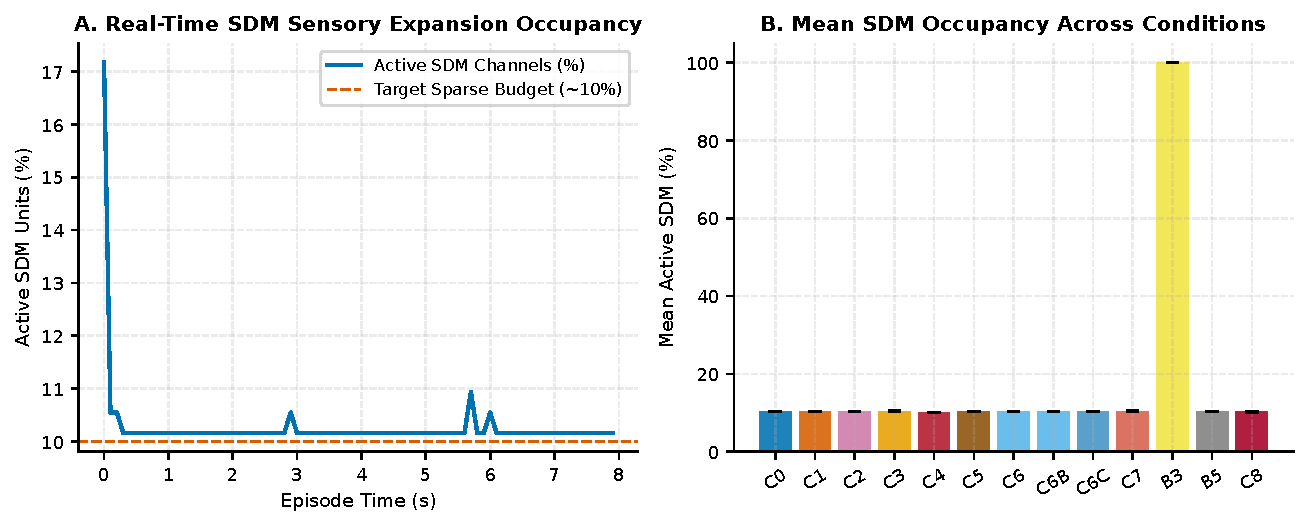
\includegraphics[width=\columnwidth]{fig03_sdm_sparse_coding.pdf}
\caption{Sparse expansion encoder occupancy across closed-loop steps (A) and conditions (B); the active budget settles at $\approx 10.2\%$ ($26/256$ units) with brief episode-onset excursions.}
\label{fig:sdm}
\end{figure}

\begin{figure}[t]
\centering
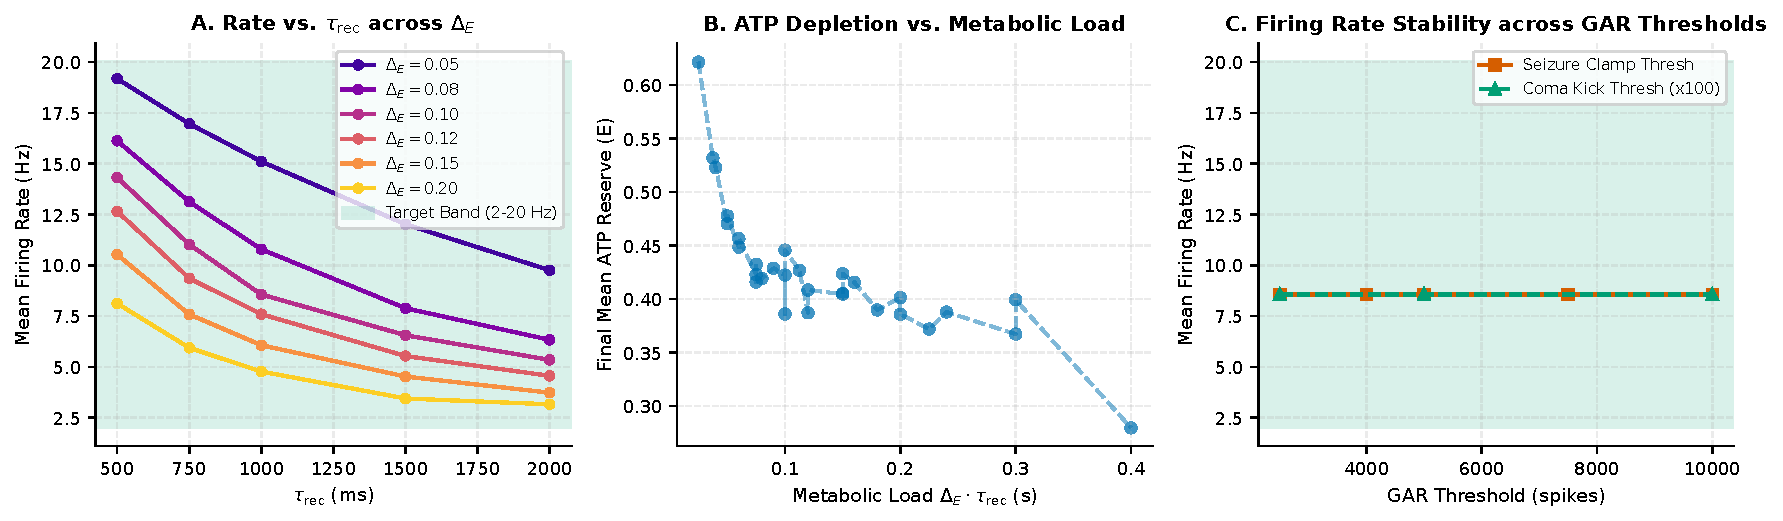
\includegraphics[width=\columnwidth]{fig13_sensitivity_sweep.pdf}
\caption{Parameter sweep: (A) mean firing rate versus $\tau_{\mathrm{rec}}$ for several $\Delta_E$; (B) final mean energy reserve versus metabolic load $\Delta_E \tau_{\mathrm{rec}}$; (C) mean rate versus GAR thresholds. $f_{\max} = 1/(\Delta_E \tau_{\mathrm{rec}})$ acts as an upper bound with finite-horizon excess.}
\label{fig:sensitivity_sweep}
\end{figure}

\end{document}
